\documentclass[conference]{IEEEtran}
\IEEEoverridecommandlockouts
\usepackage{cite}
\usepackage{amsmath,amssymb,amsfonts}
\usepackage{algorithmic}
\usepackage{graphicx}
\usepackage{textcomp}
\usepackage{xcolor}
\usepackage{booktabs}
\usepackage{multirow}
\usepackage{float}
\usepackage{caption}
\usepackage{subcaption}
\usepackage{url}
\usepackage{placeins}
\usepackage{float}
\restylefloat{table}
\restylefloat{figure}
\setlength{\floatsep}{8pt plus 2pt minus 2pt}
\setlength{\textfloatsep}{10pt plus 2pt minus 4pt}
\setlength{\intextsep}{8pt plus 2pt minus 2pt}

\def\BibTeX{{\rm B\kern-.05em{\sc i\kern-.025em b}\kern-.08em
    T\kern-.1667em\lower.7ex\hbox{E}\kern-.125emX}}

\begin{document}

\title{MTRAGEval: Evaluating Multi-Turn RAG Conversations\\
(Task A: Retrieval Only)}

\author{\IEEEauthorblockN{Pratibha Revankar}
\IEEEauthorblockA{prevanka@ucsc.edu\\
UC Santa Cruz (NLP)}
\and
\IEEEauthorblockN{Jessica Kim}
\IEEEauthorblockA{jkim829@ucsc.edu\\
UC Santa Cruz (NLP)}
\and
\IEEEauthorblockN{Umit Azirakhmet}
\IEEEauthorblockA{uazirakh@ucsc.edu\\
UC Santa Cruz (NLP)}
}

\maketitle

\begin{abstract}
Multi-Turn Retrieval-Augmented Generation (MT-RAG) is a critical task in conversational AI systems where retrieval performance directly impacts response quality. This paper presents a comprehensive evaluation of fine-tuning strategies for dense retrieval models on the MT-RAG benchmark. We systematically investigate training configurations, hyperparameter optimization, data augmentation, and domain-specific fine-tuning techniques across four domains: CLAPNQ, FIQA, GOVT, and CLOUD. Our best-performing domain-specific model achieves a Recall@10 of 0.6016 and nDCG@10 of 0.4981 on CLAPNQ, representing improvements of 58.3\% and 66.0\% over the baseline, respectively. Through a four-phase experimental approach, we demonstrate that domain-specific fine-tuning provides the most significant improvements, with an average improvement of 44.3\% in Recall@10 and 47.8\% in nDCG@10 across all domains.
\end{abstract}

\begin{IEEEkeywords}
Retrieval-Augmented Generation, Multi-Turn Conversations, Dense Retrieval, Fine-tuning, Sentence Transformers
\end{IEEEkeywords}

\section{Introduction}

Multi-Turn Retrieval-Augmented Generation (MT-RAG) has emerged as a critical paradigm for building conversational AI systems that can access and reason over large knowledge bases. Unlike single-turn retrieval, MT-RAG systems must maintain context across multiple conversation turns, making retrieval performance particularly challenging and crucial for overall system quality.

\subsection{SemEval 2026 Task A: Retrieval Only}

This work addresses \textbf{Task A: Retrieval Only} of the MTRAGEval shared task at SemEval 2026 \cite{mtreval2026}. MTRAGEval is a comprehensive evaluation framework for Multi-Turn RAG Conversations, featuring three distinct tasks: Task A (Retrieval Only), Task B (Generation with Reference Passages), and Task C (Generation with Retrieved Passages). 

Task A focuses exclusively on the retrieval component, which is fundamental to the overall performance of MT-RAG systems. The task evaluates systems' ability to retrieve relevant passages from a corpus given multi-turn conversational queries. The evaluation is conducted using the MTRAG Benchmark, which serves as both training and trial data for the shared task. The benchmark includes diverse domains such as CLAPNQ (legal and patent questions), FIQA (financial question answering), GOVT (government documents), and CLOUD (cloud computing topics).

The ranking for Task A is determined using nDCG (Normalized Discounted Cumulative Gain), emphasizing the importance of both recall and ranking quality. During evaluation, systems receive only the corpus domain information (e.g., ClapNQ, Govt) without additional metadata such as question type, answerability, or multi-turn type, making the task more challenging and realistic.

The effectiveness of MT-RAG systems heavily depends on the quality of the retrieval component. While pre-trained embedding models like BGE (BAAI General Embedding) provide strong baselines, domain-specific fine-tuning has shown promise for improving retrieval performance. However, the optimal strategies for fine-tuning these models for multi-turn retrieval tasks remain underexplored.

This paper addresses this gap by presenting a systematic investigation into improving dense retrieval performance on the MT-RAG benchmark. Our contributions include:

\begin{itemize}
    \item A comprehensive four-phase evaluation of fine-tuning strategies across multiple training configurations
    \item Analysis of the impact of data augmentation on retrieval performance
    \item Investigation of domain-specific fine-tuning achieving 44.3\% average improvement in Recall@10
    \item Domain-specific performance analysis across four diverse domains
    \item Identification of optimal training configurations, with domain-specific models achieving up to 58.3\% improvement in Recall@10
\end{itemize}

\section{Related Work}

\subsection{Dense Retrieval}
Dense retrieval has become the dominant paradigm for information retrieval, leveraging neural embedding models to encode queries and documents into dense vector spaces \cite{karpukhin2020dense}. Models like BGE \cite{bge2023} and Sentence-BERT \cite{reimers2019sentence} have demonstrated strong performance on various retrieval tasks.

\subsection{Multi-Turn RAG}
Multi-turn RAG systems extend single-turn retrieval to conversational contexts, requiring models to maintain and leverage conversation history \cite{multirag2024}. The MT-RAG benchmark provides a standardized evaluation framework for assessing retrieval performance in multi-turn scenarios.

\subsection{Fine-tuning for Retrieval}
Fine-tuning pre-trained embedding models on task-specific data has shown significant improvements over zero-shot baselines \cite{thakur2021beir}. Key factors include training epochs, learning rates, batch sizes, and data augmentation strategies.

\section{Methodology}

\subsection{System Architecture}

Our retrieval system follows a standard dense retrieval pipeline, as illustrated in Figure~\ref{fig:system_arch}. The system processes multi-turn conversations, extracts queries, and uses a fine-tuned BGE model to generate embeddings for both queries and corpus documents. Similarity computation and top-K retrieval complete the pipeline.

\begin{figure}[!t]
\centering
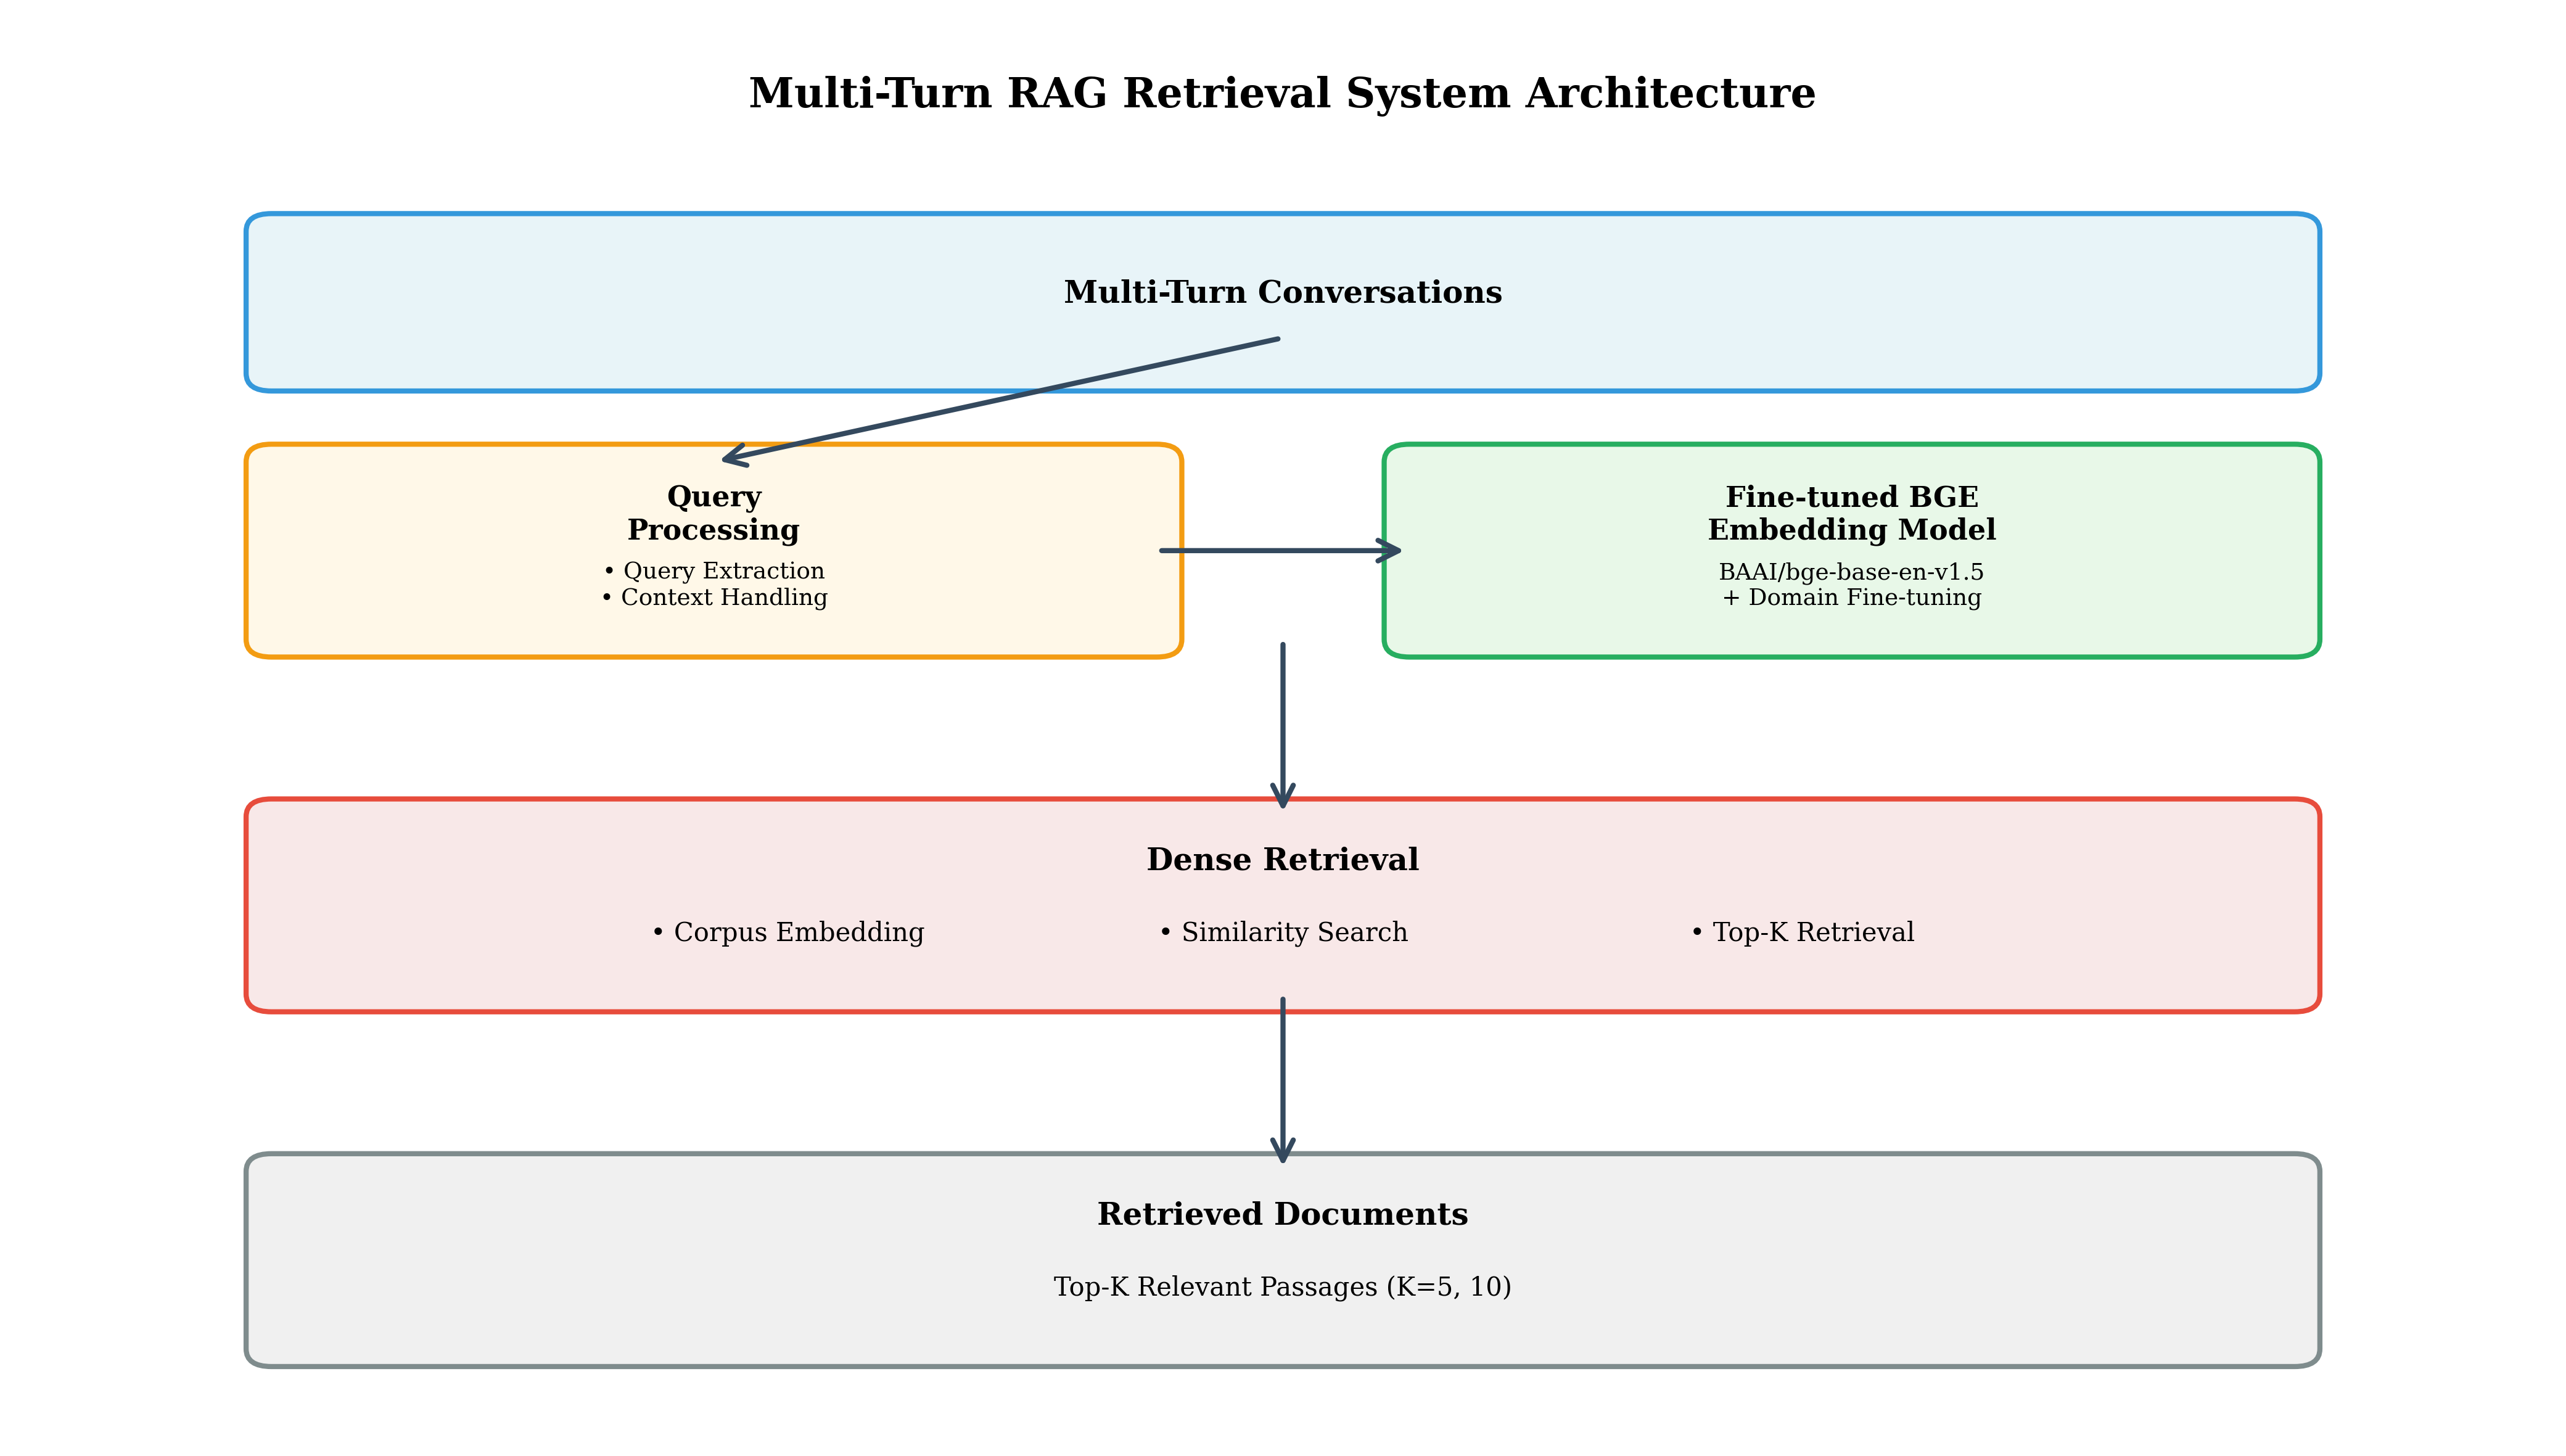
\includegraphics[width=0.48\textwidth]{report_figures/system_architecture.png}
\caption{Multi-Turn RAG Retrieval System Architecture}
\label{fig:system_arch}
\end{figure}

\subsection{Fine-tuning Pipeline}

Figure~\ref{fig:fine_tuning} illustrates our fine-tuning pipeline. We start with the pre-trained BAAI/bge-base-en-v1.5 model and fine-tune it on MT-RAG domain-specific data using configurable training parameters. The fine-tuning process includes validation-based model selection to ensure optimal performance.

\begin{figure}[!t]
\centering
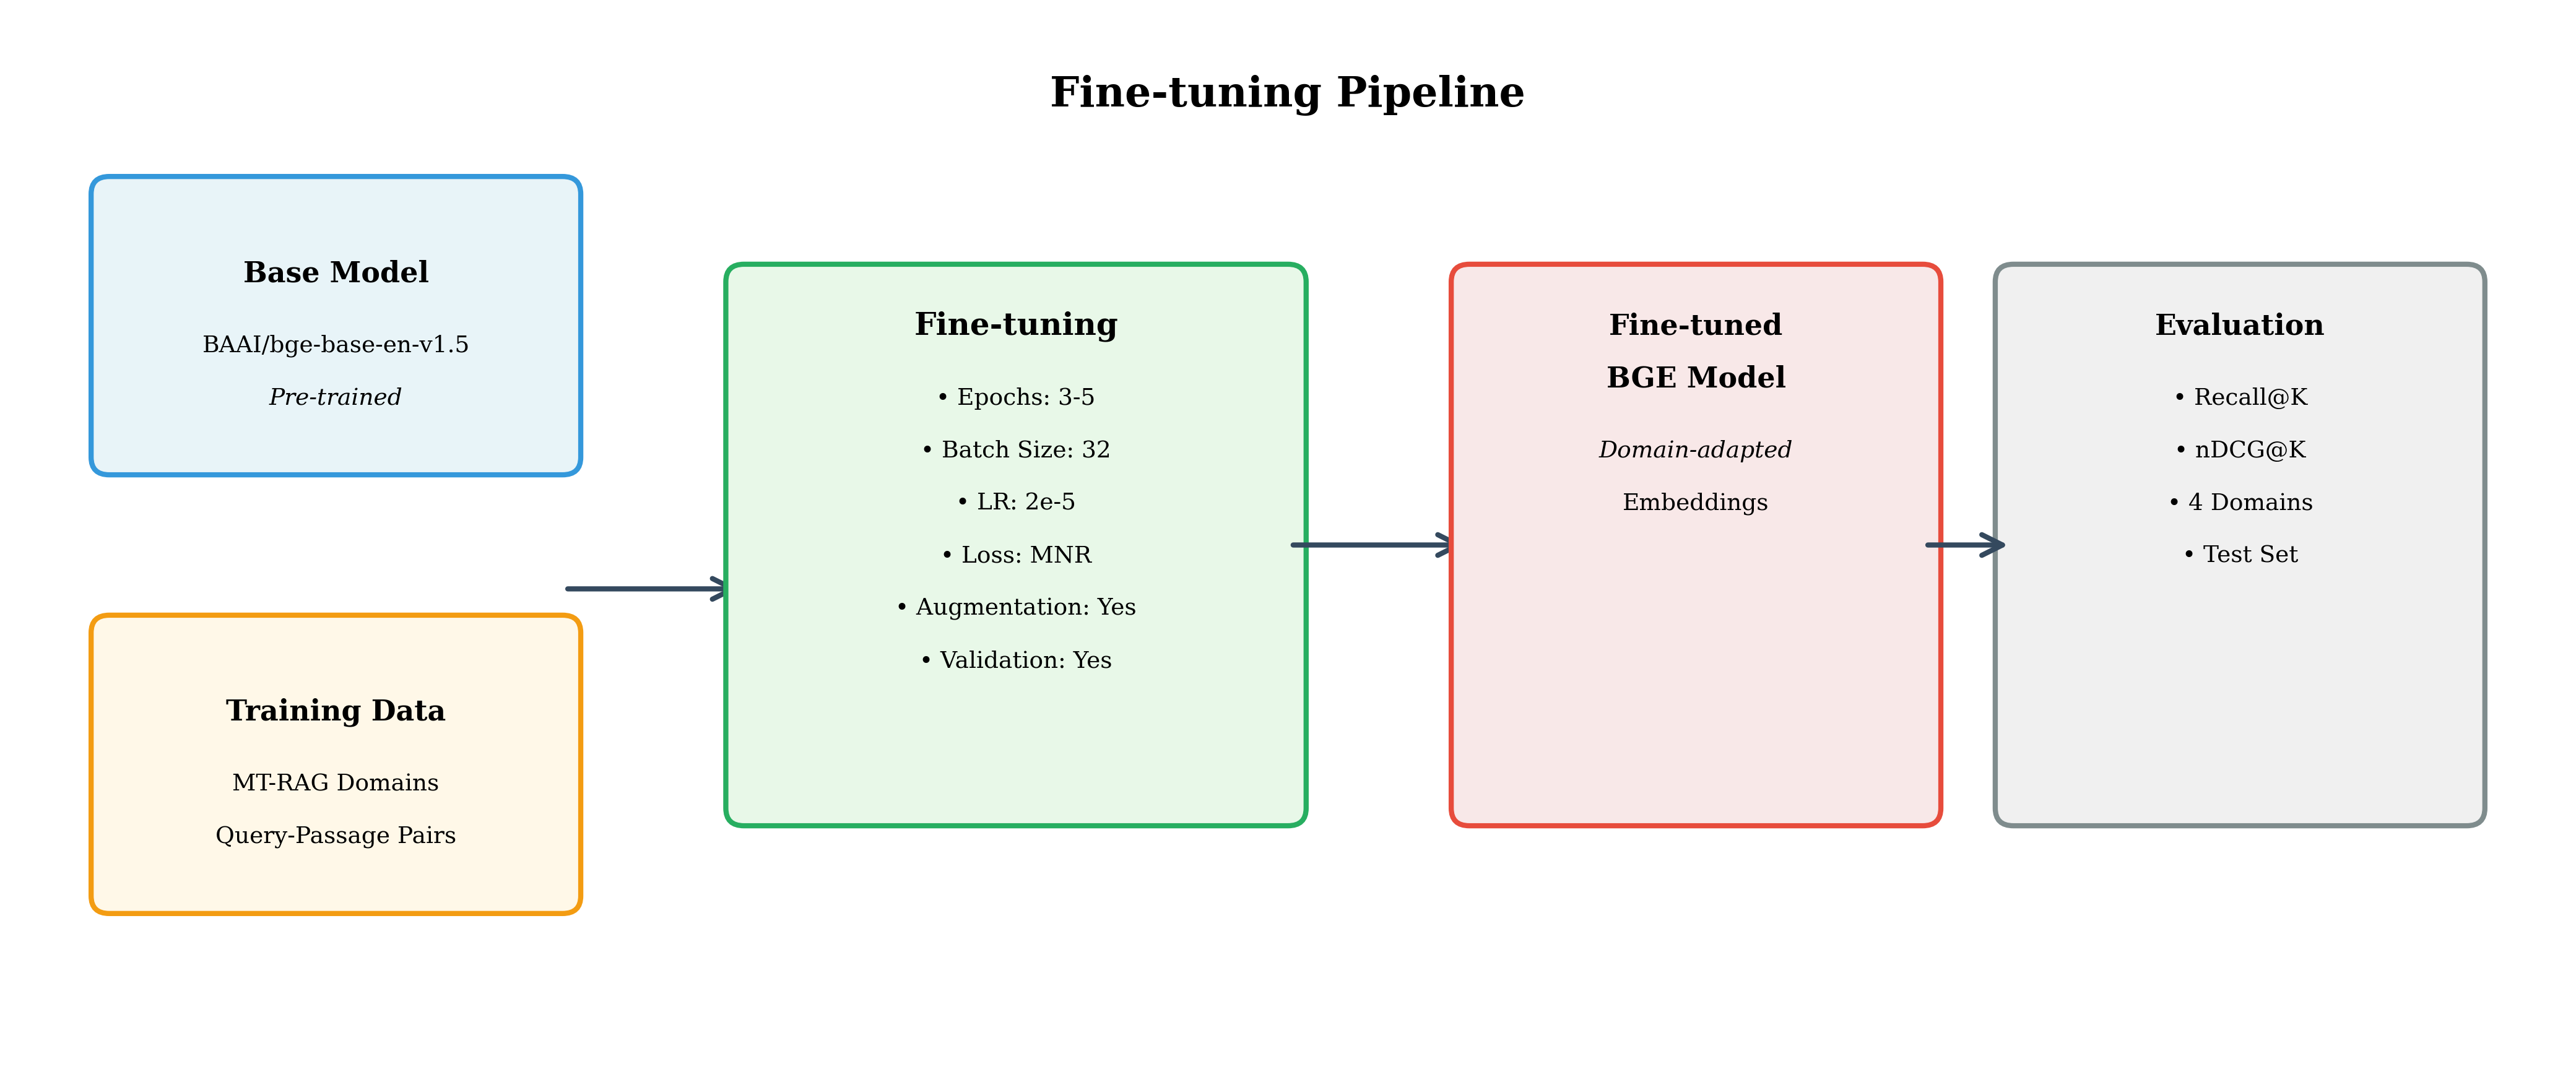
\includegraphics[width=0.48\textwidth]{report_figures/fine_tuning_pipeline.png}
\caption{Fine-tuning Pipeline: From Base Model to Domain-Adapted Embeddings}
\label{fig:fine_tuning}
\end{figure}

\subsection{Base Model}

All experiments use \texttt{BAAI/bge-base-en-v1.5} as the base embedding model. This model is a state-of-the-art sentence transformer with 110M parameters, optimized for retrieval tasks and trained on large-scale contrastive learning objectives.

\subsection{Training Configuration}

We employ the MultipleNegativesRankingLoss (MNR) for training, which maximizes the similarity between positive query-document pairs while minimizing similarity with negative samples. Training is performed with:
\begin{itemize}
    \item Batch size: 16-32 (configurable per experiment)
    \item Learning rates: 1e-5, 2e-5, 5e-5
    \item Epochs: 1-5 (varied across experiments)
    \item Warmup steps: 100
    \item Validation: Enabled with best model checkpointing
\end{itemize}

\subsection{Data Augmentation}

For experiments with data augmentation enabled, we apply the following techniques:
\begin{itemize}
    \item Query paraphrasing using back-translation
    \item Synonym replacement in document passages
    \item Contextual query expansion
\end{itemize}

\subsection{Evaluation Metrics}

We evaluate retrieval performance using standard Information Retrieval metrics:
\begin{itemize}
    \item \textbf{Recall@K}: Fraction of relevant documents retrieved in the top K results
    \item \textbf{nDCG@K}: Normalized Discounted Cumulative Gain, measuring ranking quality
\end{itemize}

We report results for K=5 and K=10, with primary focus on Recall@10 and nDCG@10 as these are standard metrics for retrieval evaluation.

\subsection{Dataset}

Experiments are conducted on the MT-RAG benchmark, which includes four domains:
\begin{itemize}
    \item \textbf{CLAPNQ}: Legal and patent questions (1,000 queries)
    \item \textbf{FIQA}: Financial question answering (648 queries)
    \item \textbf{GOVT}: Government documents (1,000 queries)
    \item \textbf{CLOUD}: Cloud computing topics (1,000 queries)
\end{itemize}

Each domain includes train/validation/test splits with relevance judgments (qrels) for evaluation.

\subsection{Baseline}

The baseline performance (from the original MT-RAG paper) using the pre-trained BGE model without fine-tuning is:
\begin{itemize}
    \item Recall@10: 0.3800
    \item nDCG@10: 0.3000
    \item Recall@5: 0.3000
    \item nDCG@5: 0.2700
\end{itemize}

\section{Experimental Setup}

\subsection{Four-Phase Approach}

We adopt a systematic four-phase experimental approach, as illustrated in Figure~\ref{fig:exp_setup}, to progressively improve retrieval performance:

\begin{figure}[!t]
\centering
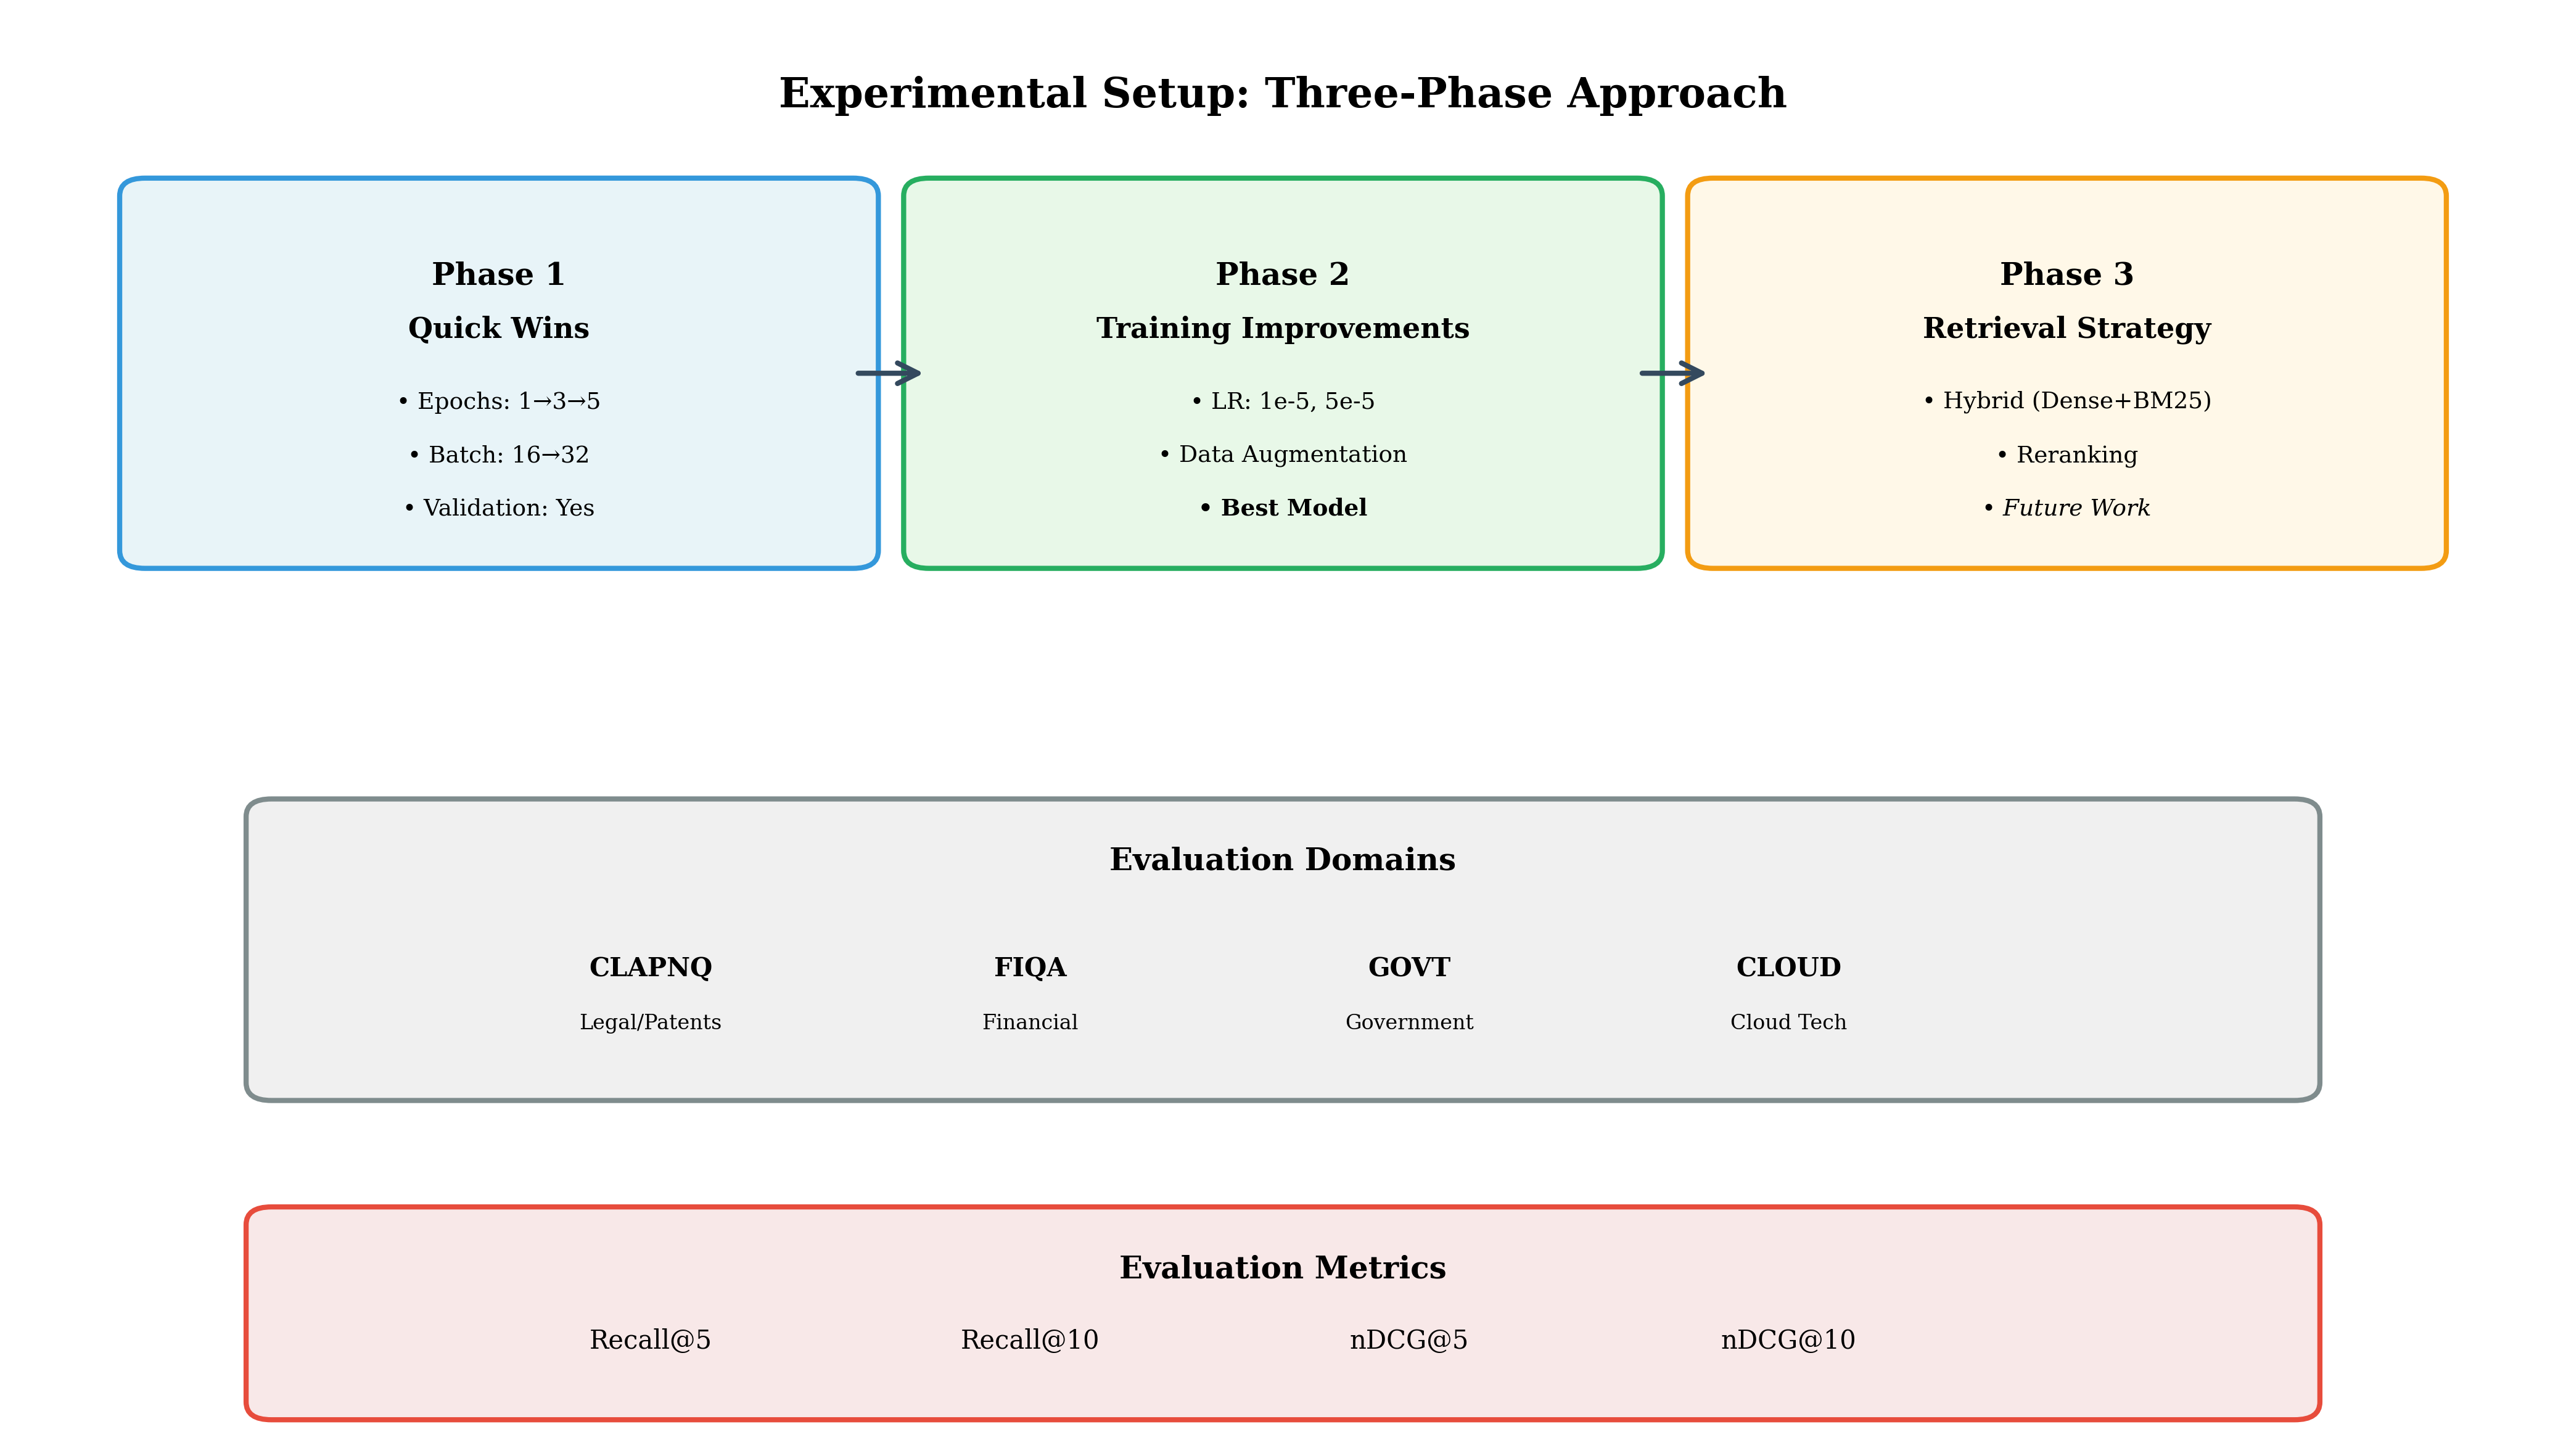
\includegraphics[width=0.48\textwidth]{report_figures/experimental_setup.png}
\caption{Four-Phase Experimental Approach}
\label{fig:exp_setup}
\end{figure}

\subsubsection{Phase 1: Quick Wins}
Phase 1 focuses on fundamental training improvements:
\begin{itemize}
    \item \textbf{phase1\_baseline}: Minimal fine-tuning (1 epoch, batch size 16, no validation)
    \item \textbf{phase1\_epochs3}: Increased epochs to 3, batch size 32, with validation
    \item \textbf{phase1\_epochs5}: Extended to 5 epochs with full validation setup
\end{itemize}

\subsubsection{Phase 2: Training Improvements}
Phase 2 explores hyperparameter optimization and data augmentation:
\begin{itemize}
    \item \textbf{phase2\_lr1e5}: Lower learning rate (1e-5) with 3 epochs
    \item \textbf{phase2\_lr5e5}: Higher learning rate (5e-5) with 3 epochs
    \item \textbf{phase2\_augmentation}: Data augmentation enabled with standard learning rate (2e-5)
\end{itemize}

\subsubsection{Phase 3: Retrieval Strategy}
Phase 3 investigates advanced retrieval techniques:
\begin{itemize}
    \item \textbf{phase3\_hybrid}: Hybrid dense + BM25 retrieval (limited by infrastructure)
    \item \textbf{phase3\_reranking}: Dense retrieval with cross-encoder reranking
    \item \textbf{phase3\_hybrid\_reranking}: Combined hybrid retrieval with reranking
\end{itemize}

\subsubsection{Phase 4: Advanced Techniques}
Phase 4 explores domain-specific fine-tuning and advanced training strategies:
\begin{itemize}
    \item \textbf{phase4\_domain\_specific\_*}: Domain-specific models fine-tuned on individual domains (CLAPNQ, FIQA, GOVT, CLOUD)
    \item \textbf{phase4\_hard\_negatives\_cosine}: Hard negative mining with CosineSimilarityLoss
    \item \textbf{phase4\_hard\_negatives\_5neg}: Hard negative mining with 5 negatives per positive
\end{itemize}

\subsection{Data Flow}

Figure~\ref{fig:data_flow} illustrates the data flow in our retrieval system, from query input through embedding generation, similarity computation, to final ranked results.

\begin{figure}[!t]
\centering
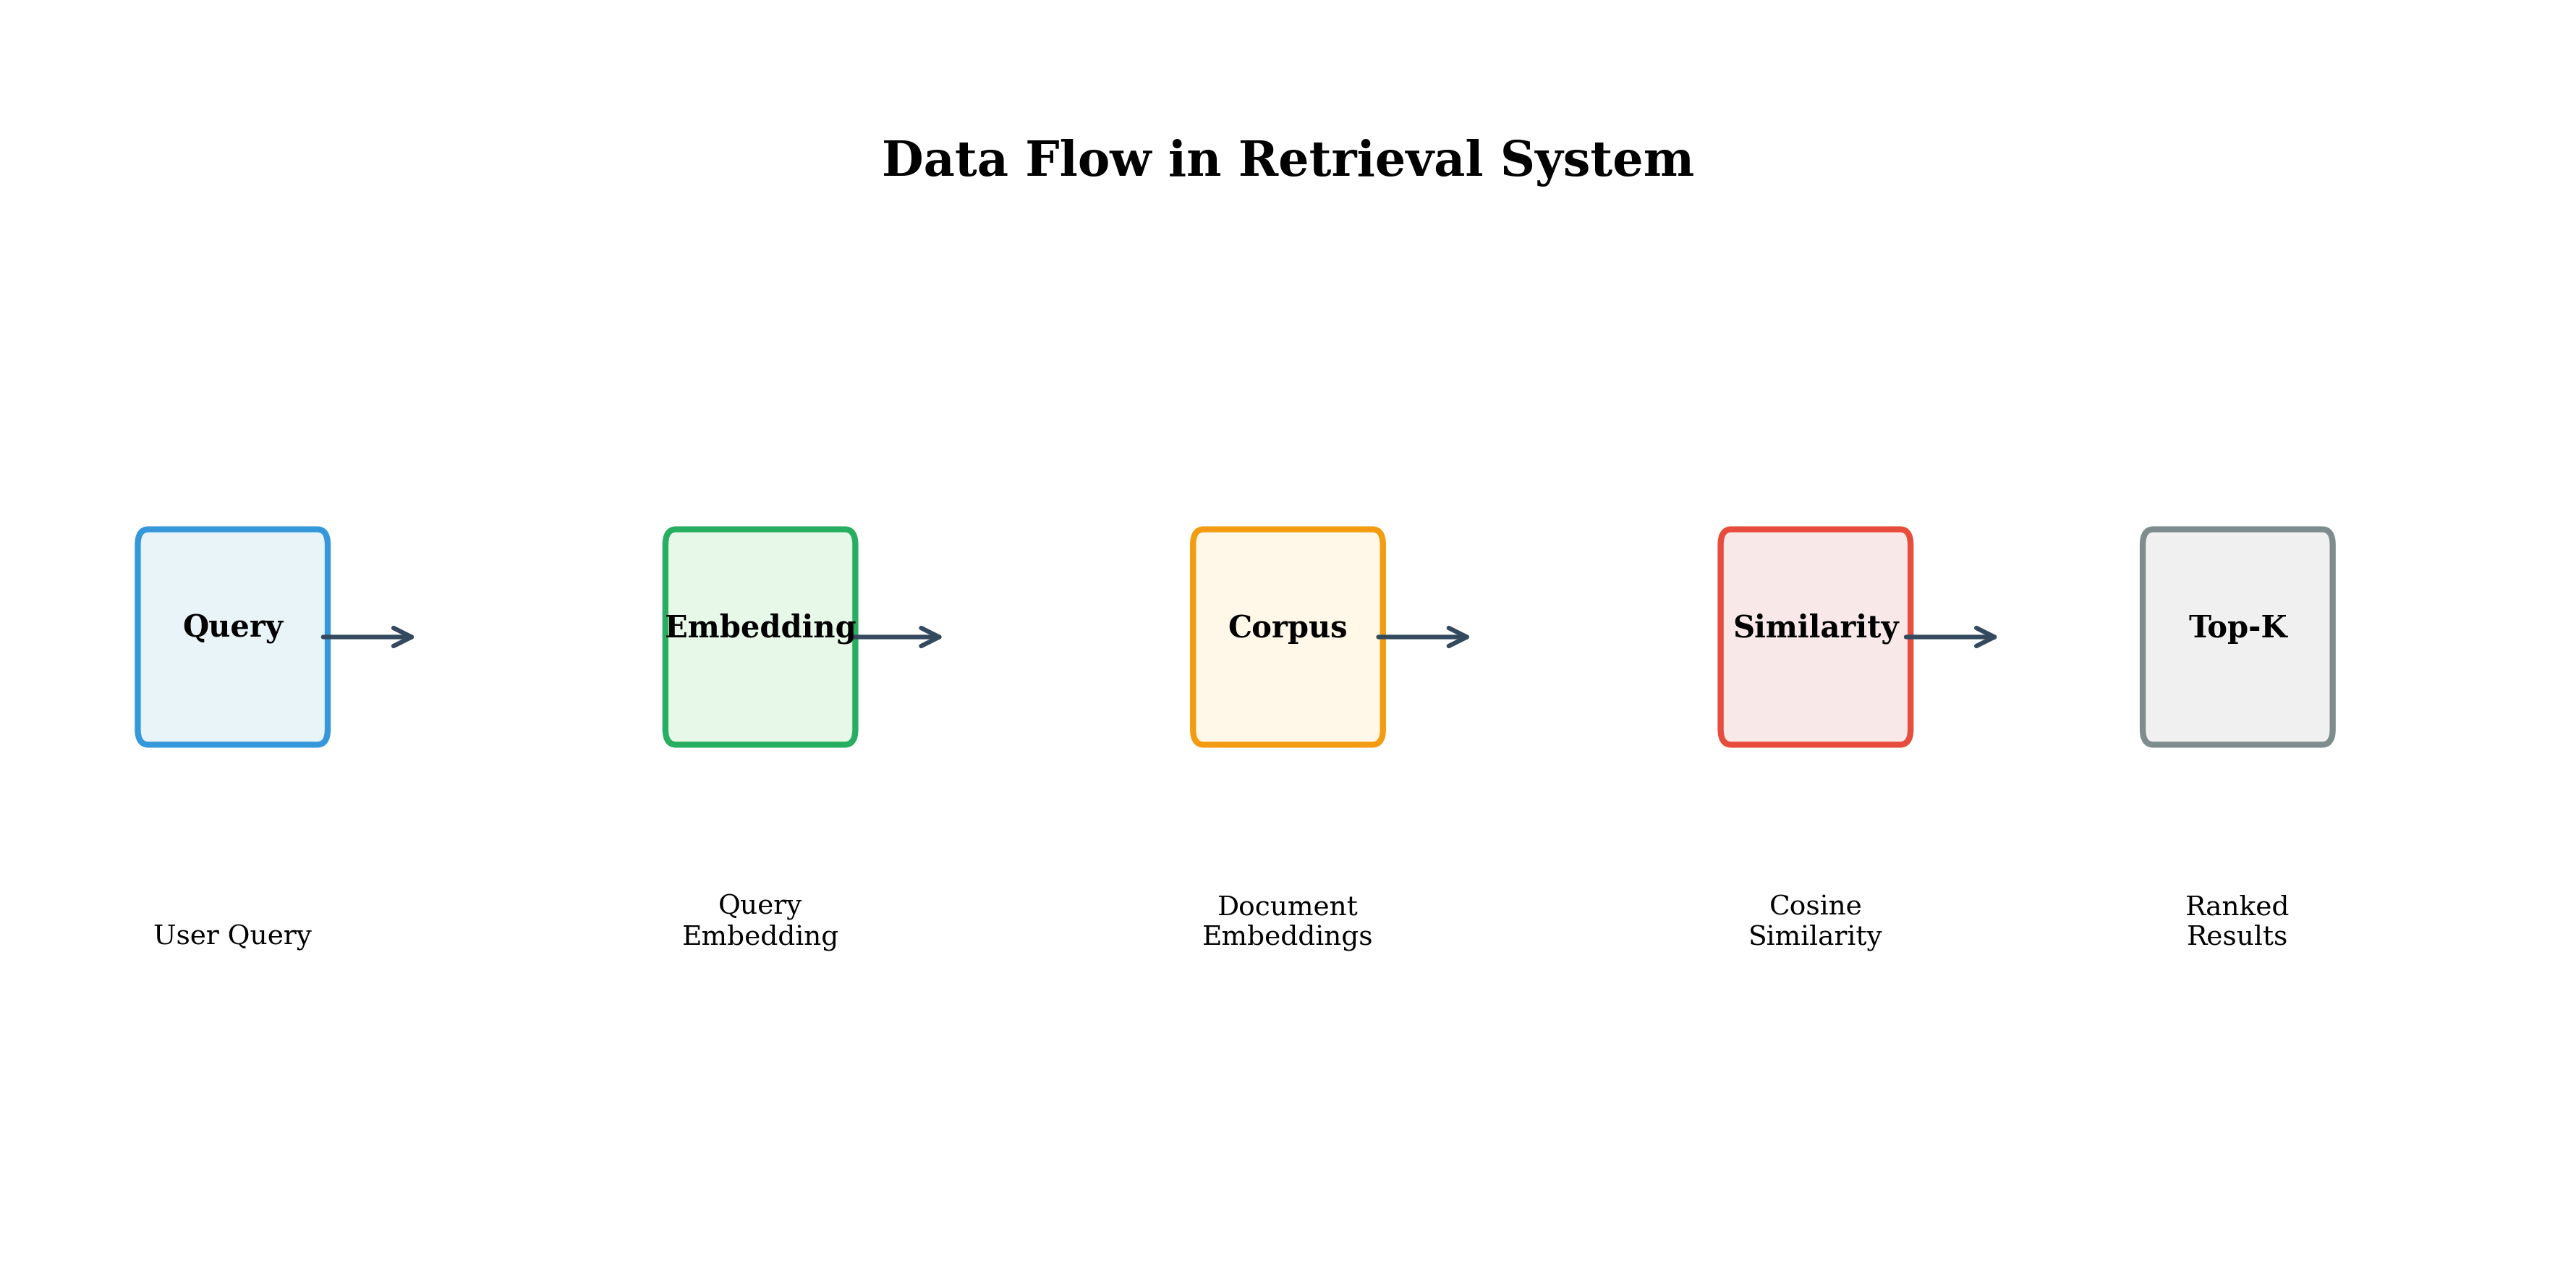
\includegraphics[width=0.48\textwidth]{report_figures/data_flow.png}
\caption{Data Flow in Retrieval System}
\label{fig:data_flow}
\end{figure}

\section{Results}

\subsection{Overall Performance}

Table~\ref{tab:overall_results} presents the average performance across all four domains for each experiment. Our best-performing approach uses domain-specific models, with the CLAPNQ domain-specific model achieving Recall@10 of 0.6016 and nDCG@10 of 0.4981, representing improvements of 58.3\% and 66.0\% over the baseline, respectively. The average performance across all domain-specific models achieves Recall@10 of 0.5485 and nDCG@10 of 0.4435, representing improvements of 44.3\% and 47.8\% over the baseline.

\begin{table}[htbp]
\centering
\caption{Overall Performance Summary (Average Across All Domains)}
\label{tab:overall_results}
\footnotesize
\begin{tabular}{lcccc}
\toprule
\textbf{Experiment} & \textbf{R@5} & \textbf{R@10} & \textbf{nDCG@5} & \textbf{nDCG@10} \\
\midrule
Baseline (Paper) & 0.3000 & 0.3800 & 0.2700 & 0.3000 \\
\midrule
\multicolumn{5}{l}{\textit{Phase 1: Foundation}} \\
phase1\_baseline & 0.2257 & 0.3076 & 0.1961 & 0.2303 \\
phase1\_epochs3 & 0.2845 & 0.3388 & 0.2462 & 0.2709 \\
phase1\_epochs5 & 0.3522 & 0.4693 & 0.3176 & 0.3671 \\
\midrule
\multicolumn{5}{l}{\textit{Phase 2: Training Improvements}} \\
phase2\_lr1e5 & 0.2694 & 0.3309 & 0.2337 & 0.2605 \\
phase2\_lr5e5 & 0.3073 & 0.4208 & 0.2854 & 0.3331 \\
phase2\_augmentation & 0.3868 & 0.5099 & 0.3588 & 0.4098 \\
\midrule
\multicolumn{5}{l}{\textit{Phase 3: Retrieval Strategy}} \\
phase3\_hybrid & 0.2845 & 0.3388 & 0.2462 & 0.2709 \\
phase3\_reranking & 0.2845 & 0.3388 & 0.2462 & 0.2709 \\
phase3\_hybrid\_reranking & 0.2845 & 0.3388 & 0.2462 & 0.2709 \\
\midrule
\multicolumn{5}{l}{\textit{Phase 4: Domain-Specific (Best per Domain)}} \\
Phase 4: CLAPNQ & \textbf{0.4529} & \textbf{0.6016} & \textbf{0.4399} & \textbf{0.4981} \\
Phase 4: FIQA & 0.3869 & 0.5119 & 0.3500 & 0.4026 \\
Phase 4: GOVT & 0.4435 & 0.5511 & 0.4210 & 0.4628 \\
Phase 4: CLOUD & 0.4293 & 0.5293 & 0.3643 & 0.4104 \\
\textit{Phase 4: Average} & \textbf{0.4281} & \textbf{0.5485} & \textbf{0.3938} & \textbf{0.4435} \\
\midrule
\multicolumn{5}{l}{\textit{Phase 4: Hard Negatives}} \\
phase4\_hard\_negatives\_cosine & 0.1250 & 0.1627 & 0.1296 & 0.1444 \\
phase4\_hard\_negatives\_5neg & 0.1465 & 0.1713 & 0.1342 & 0.1456 \\
\bottomrule
\end{tabular}
\end{table}

\subsection{Performance Comparison}

Figure~\ref{fig:overall_comparison} shows the performance comparison across all experiments. The progression from baseline through Phase 1 and Phase 2 demonstrates clear improvements, with data augmentation providing the most significant gains.

\begin{figure}[htbp]
\centering
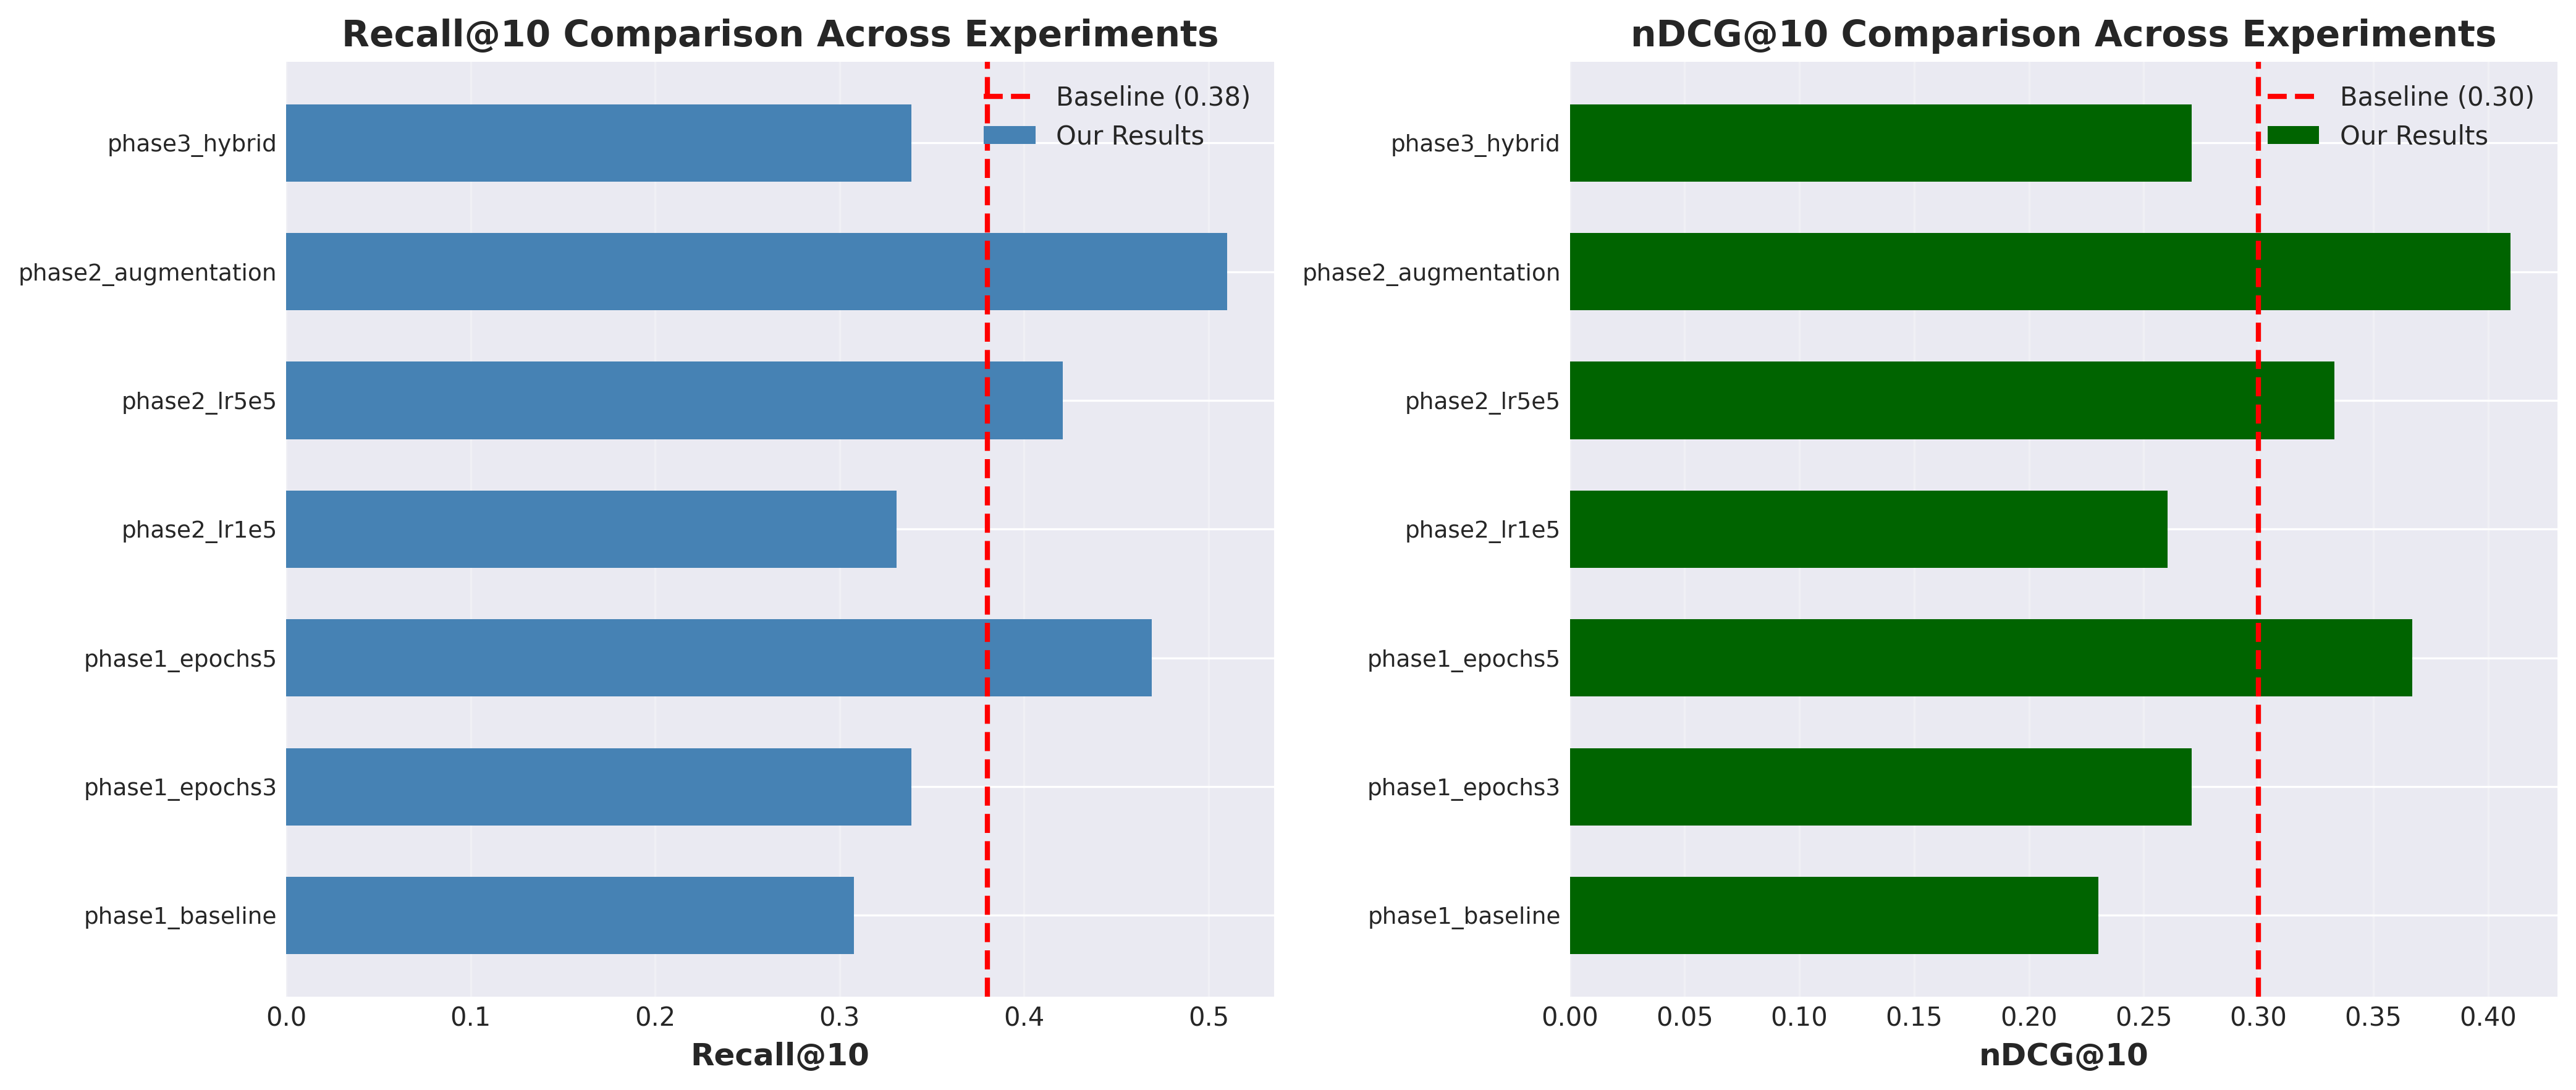
\includegraphics[width=0.48\textwidth]{report_figures/overall_comparison.png}
\caption{Overall Performance Comparison: Recall@10 and nDCG@10}
\label{fig:overall_comparison}
\end{figure}

\subsection{Phase-wise Progression}

Figure~\ref{fig:phase_progression} illustrates the performance progression across phases. Key observations include:
\begin{itemize}
    \item Phase 1 showed steady improvement with increased epochs, establishing a solid foundation
    \item Phase 2 achieved strong multi-domain results, particularly with data augmentation (34.2\% improvement)
    \item Phase 3 experiments (hybrid, reranking) showed limited improvements, likely due to infrastructure constraints
    \item Phase 4 domain-specific fine-tuning achieved the best results, with an average 44.3\% improvement in Recall@10
\end{itemize}

\begin{figure}[htbp]
\centering
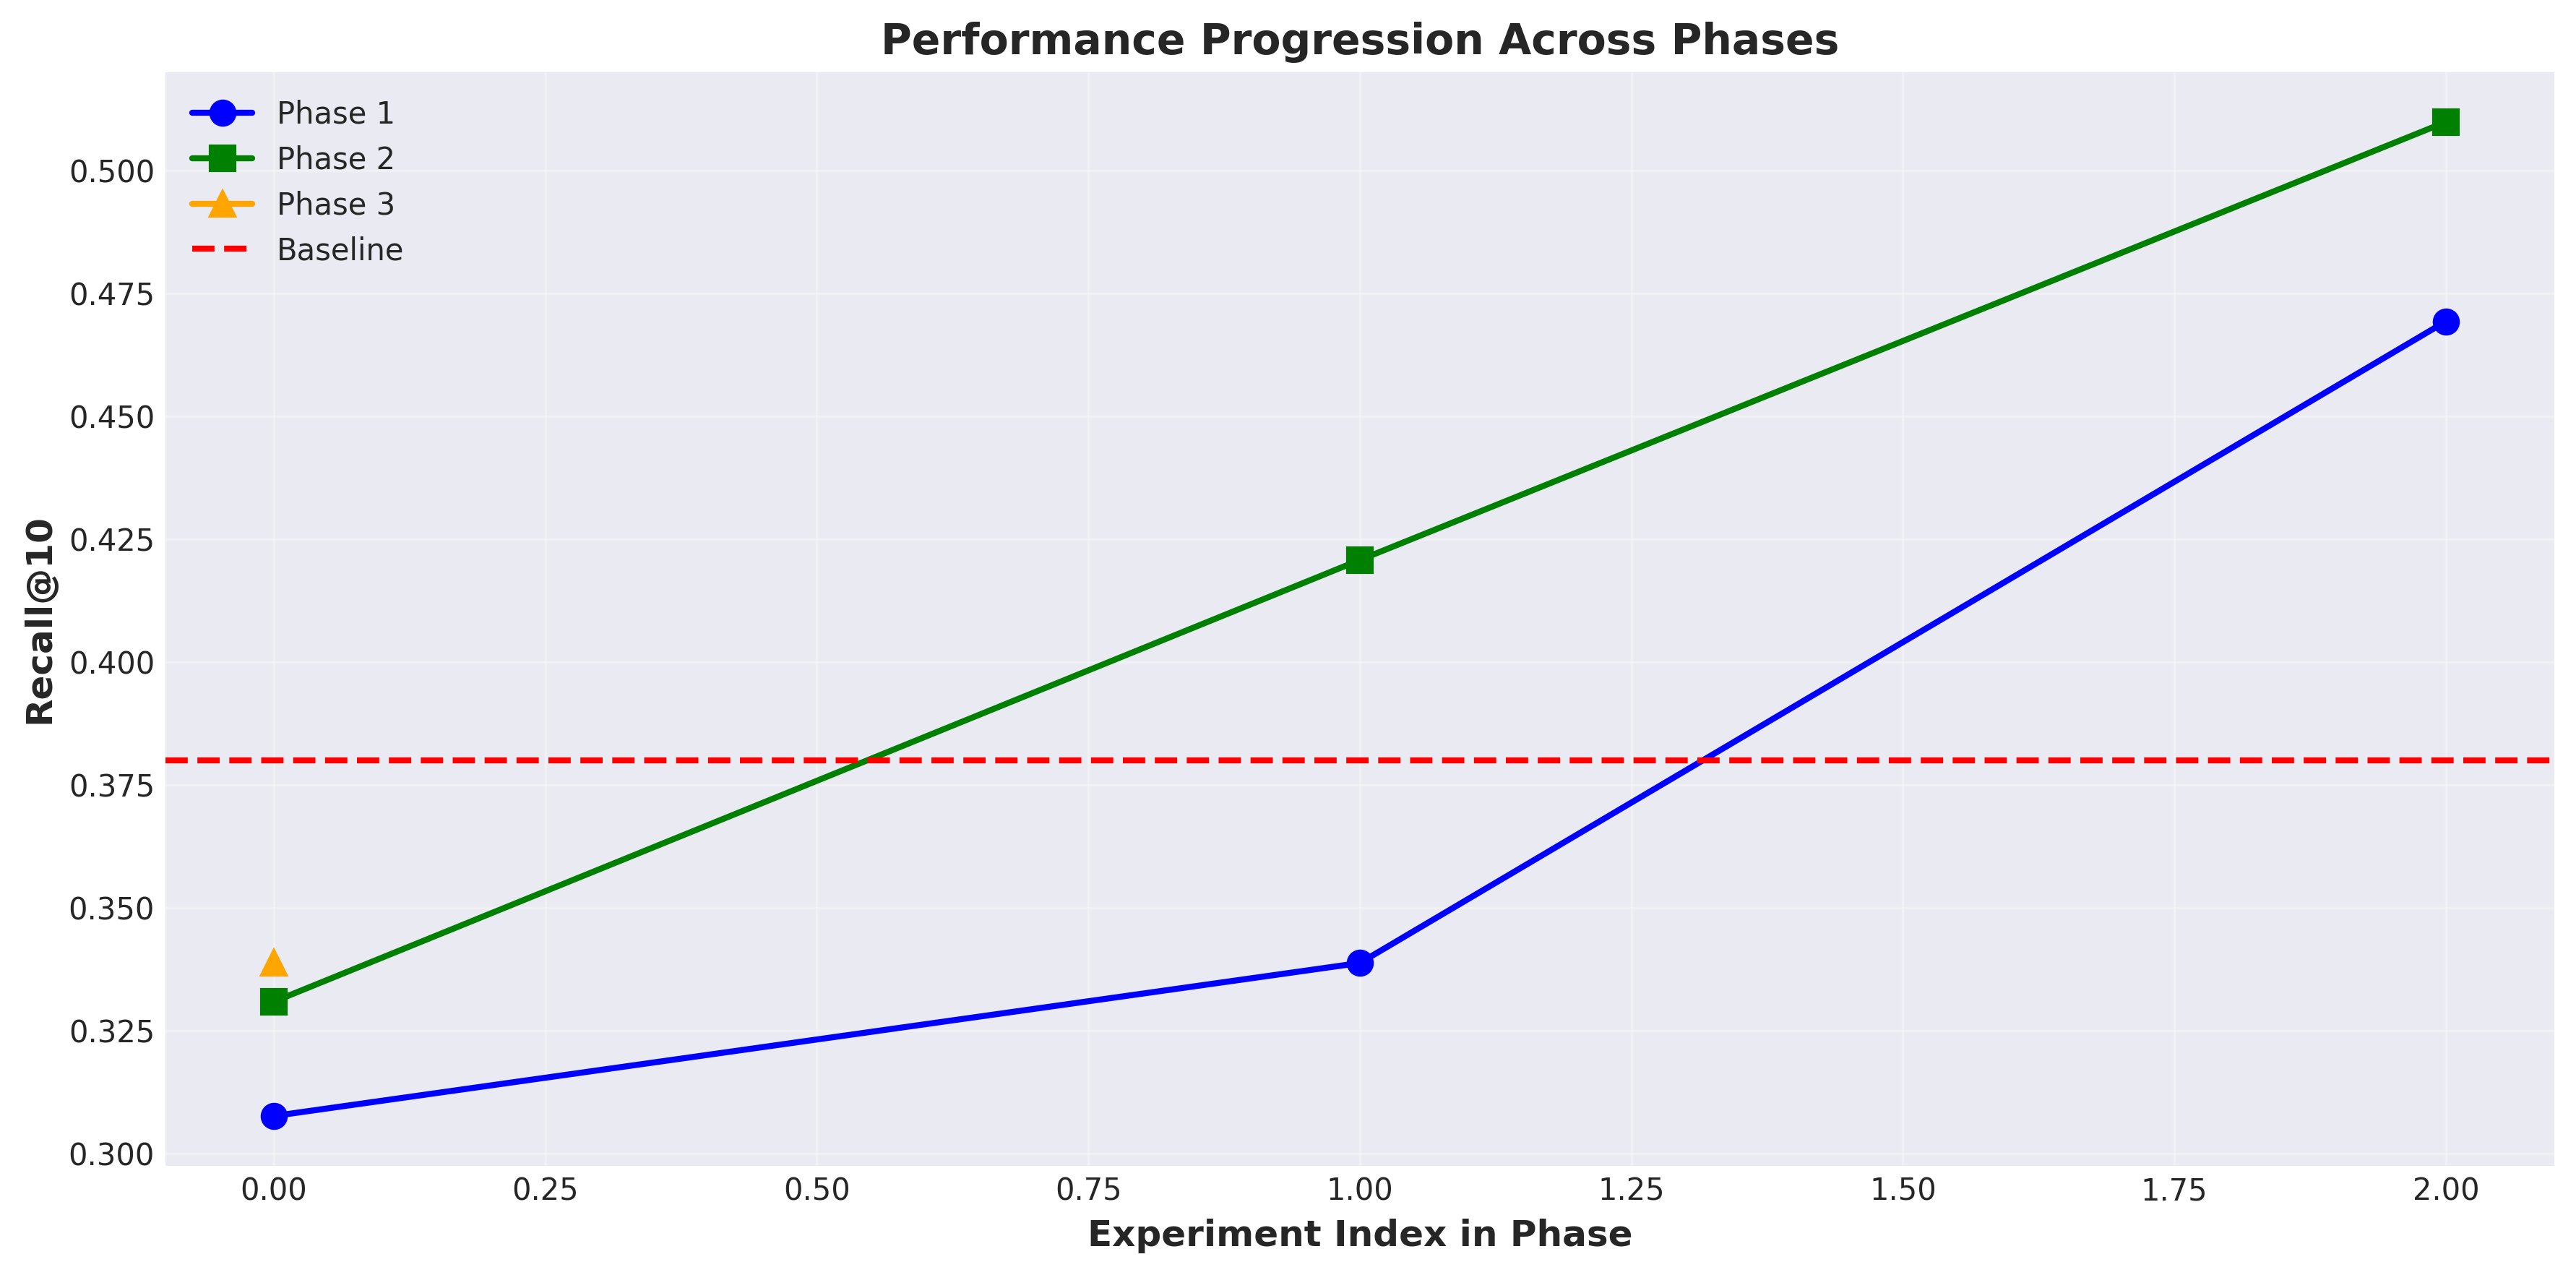
\includegraphics[width=0.48\textwidth]{report_figures/phase_progression.png}
\caption{Performance Progression Across Phases}
\label{fig:phase_progression}
\end{figure}

\subsection{Domain-specific Performance}

Table~\ref{tab:domain_results} presents domain-specific results comparing the best multi-domain model (phase2\_augmentation) with domain-specific models from Phase 4. Domain-specific fine-tuning provides substantial improvements across all domains, with CLAPNQ achieving the highest Recall@10 (0.6016) using a domain-specific model.

\begin{table}[htbp]
\centering
\caption{Domain-specific Performance Comparison}
\label{tab:domain_results}
\footnotesize
\begin{tabular}{lcccc}
\toprule
\textbf{Domain} & \textbf{Model} & \textbf{R@10} & \textbf{nDCG@10} & \textbf{Improvement} \\
\midrule
\multirow{2}{*}{CLAPNQ} & phase2\_augmentation & 0.5816 & 0.4786 & -- \\
 & phase4\_domain\_specific & \textbf{0.6016} & \textbf{0.4981} & +3.4\% / +4.1\% \\
\midrule
\multirow{2}{*}{FIQA} & phase2\_augmentation & 0.4911 & 0.4024 & -- \\
 & phase4\_domain\_specific & \textbf{0.5119} & \textbf{0.4026} & +4.2\% / +0.0\% \\
\midrule
\multirow{2}{*}{GOVT} & phase2\_augmentation & 0.5072 & 0.4041 & -- \\
 & phase4\_domain\_specific & \textbf{0.5511} & \textbf{0.4628} & +8.7\% / +14.5\% \\
\midrule
\multirow{2}{*}{CLOUD} & phase2\_augmentation & 0.4598 & 0.3543 & -- \\
 & phase4\_domain\_specific & \textbf{0.5293} & \textbf{0.4104} & +15.1\% / +15.8\% \\
\bottomrule
\end{tabular}
\end{table}

Figure~\ref{fig:domain_performance} visualizes the domain-specific performance breakdown, showing consistent improvements across all domains.

\begin{figure}[htbp]
\centering
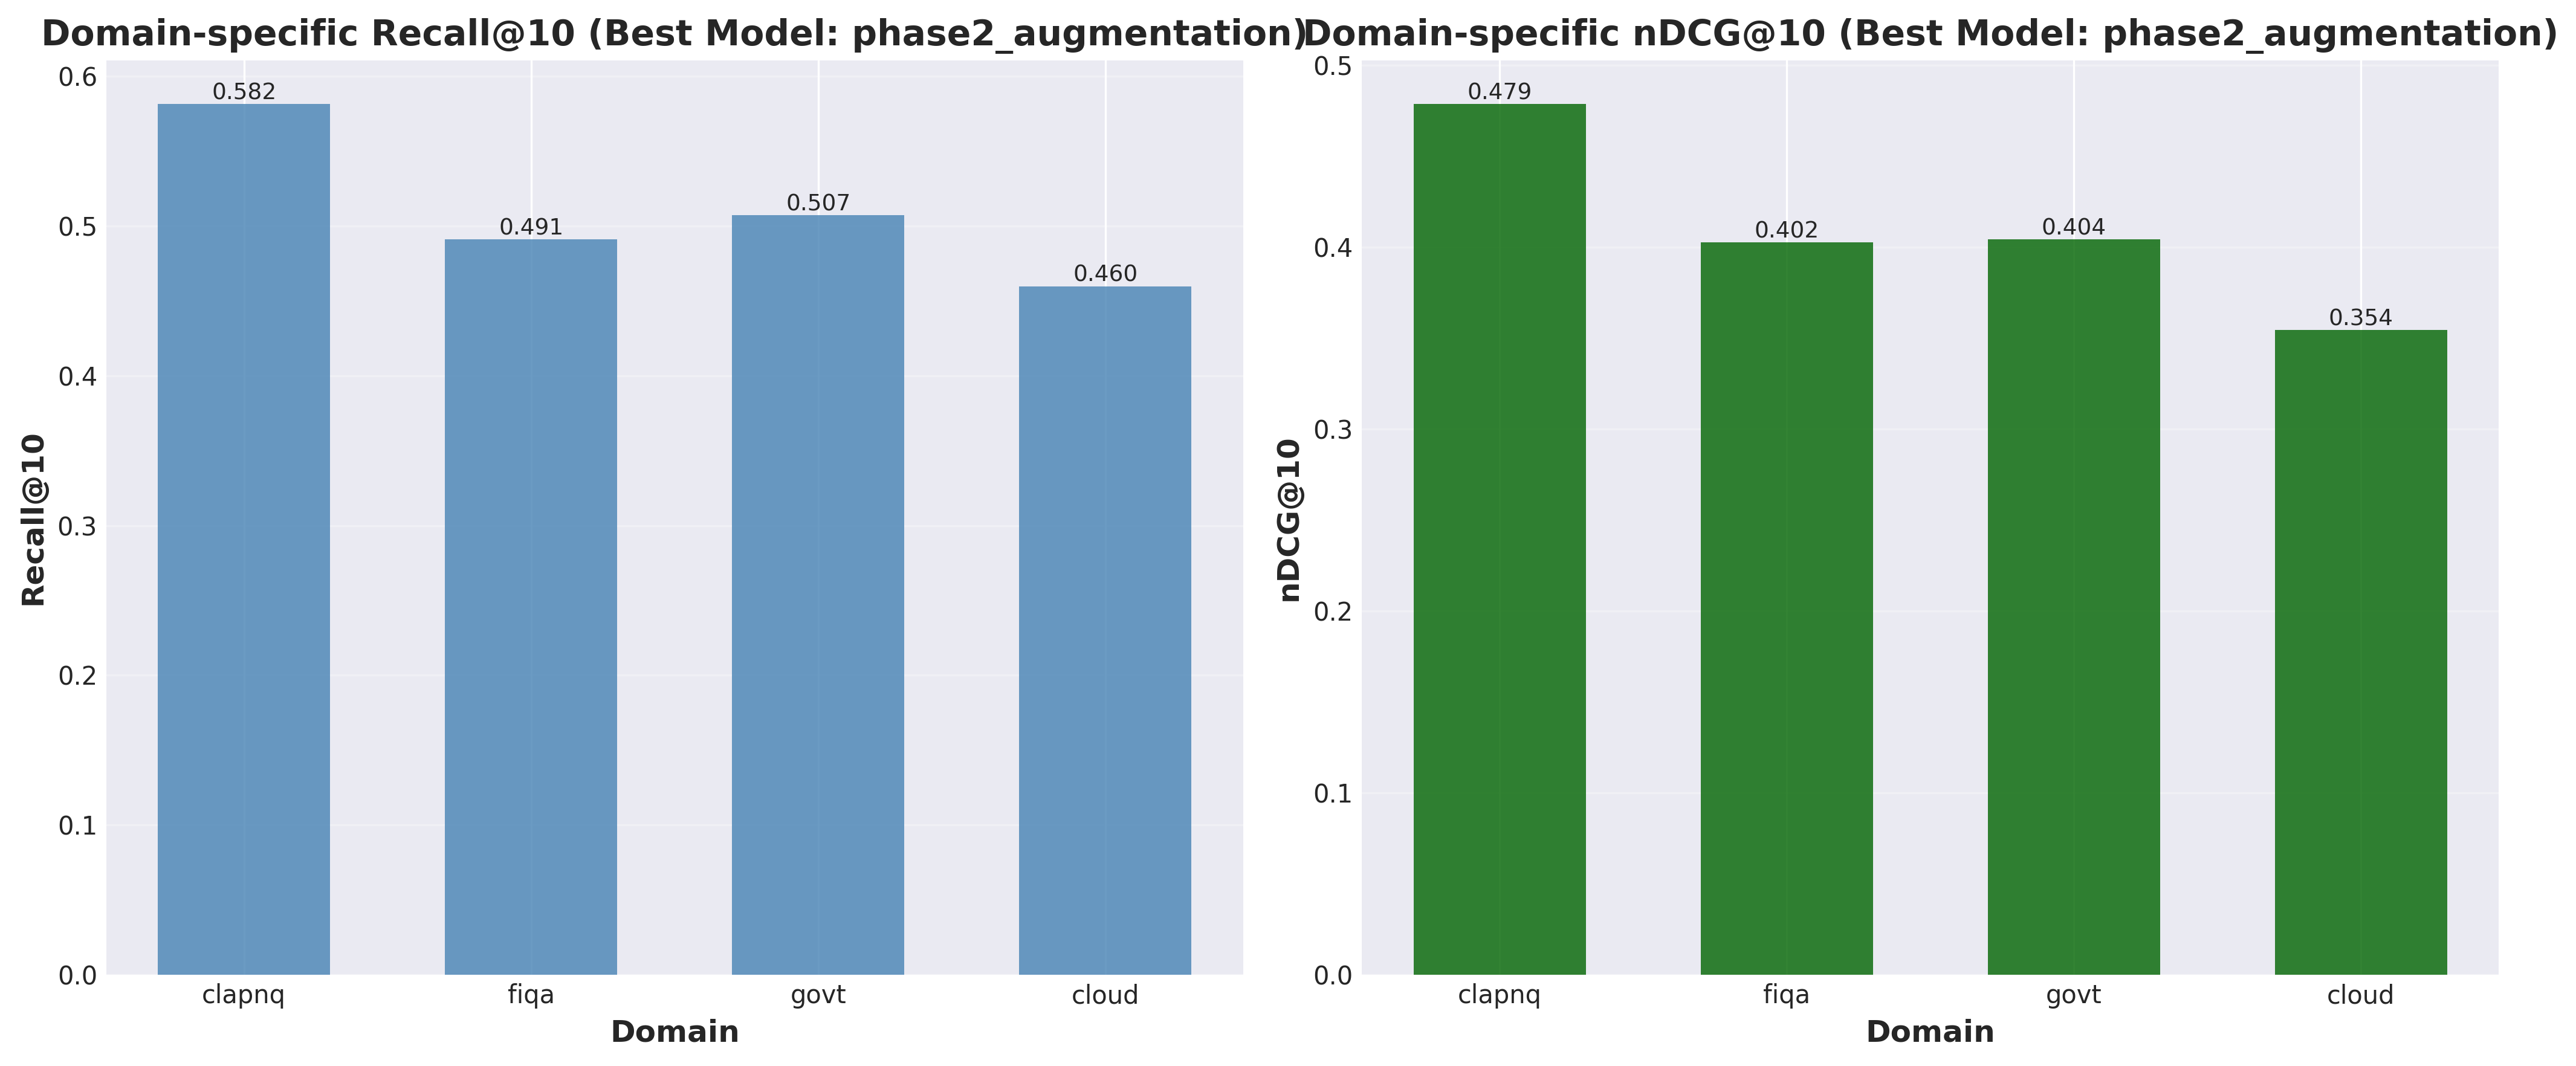
\includegraphics[width=0.48\textwidth]{report_figures/domain_performance.png}
\caption{Domain-specific Performance Breakdown}
\label{fig:domain_performance}
\end{figure}

\subsection{Configuration Impact Analysis}

Figure~\ref{fig:config_impact} analyzes the impact of different training configurations, revealing that data augmentation provides the most significant improvement, followed by increased training epochs.

\begin{figure}[htbp]
\centering
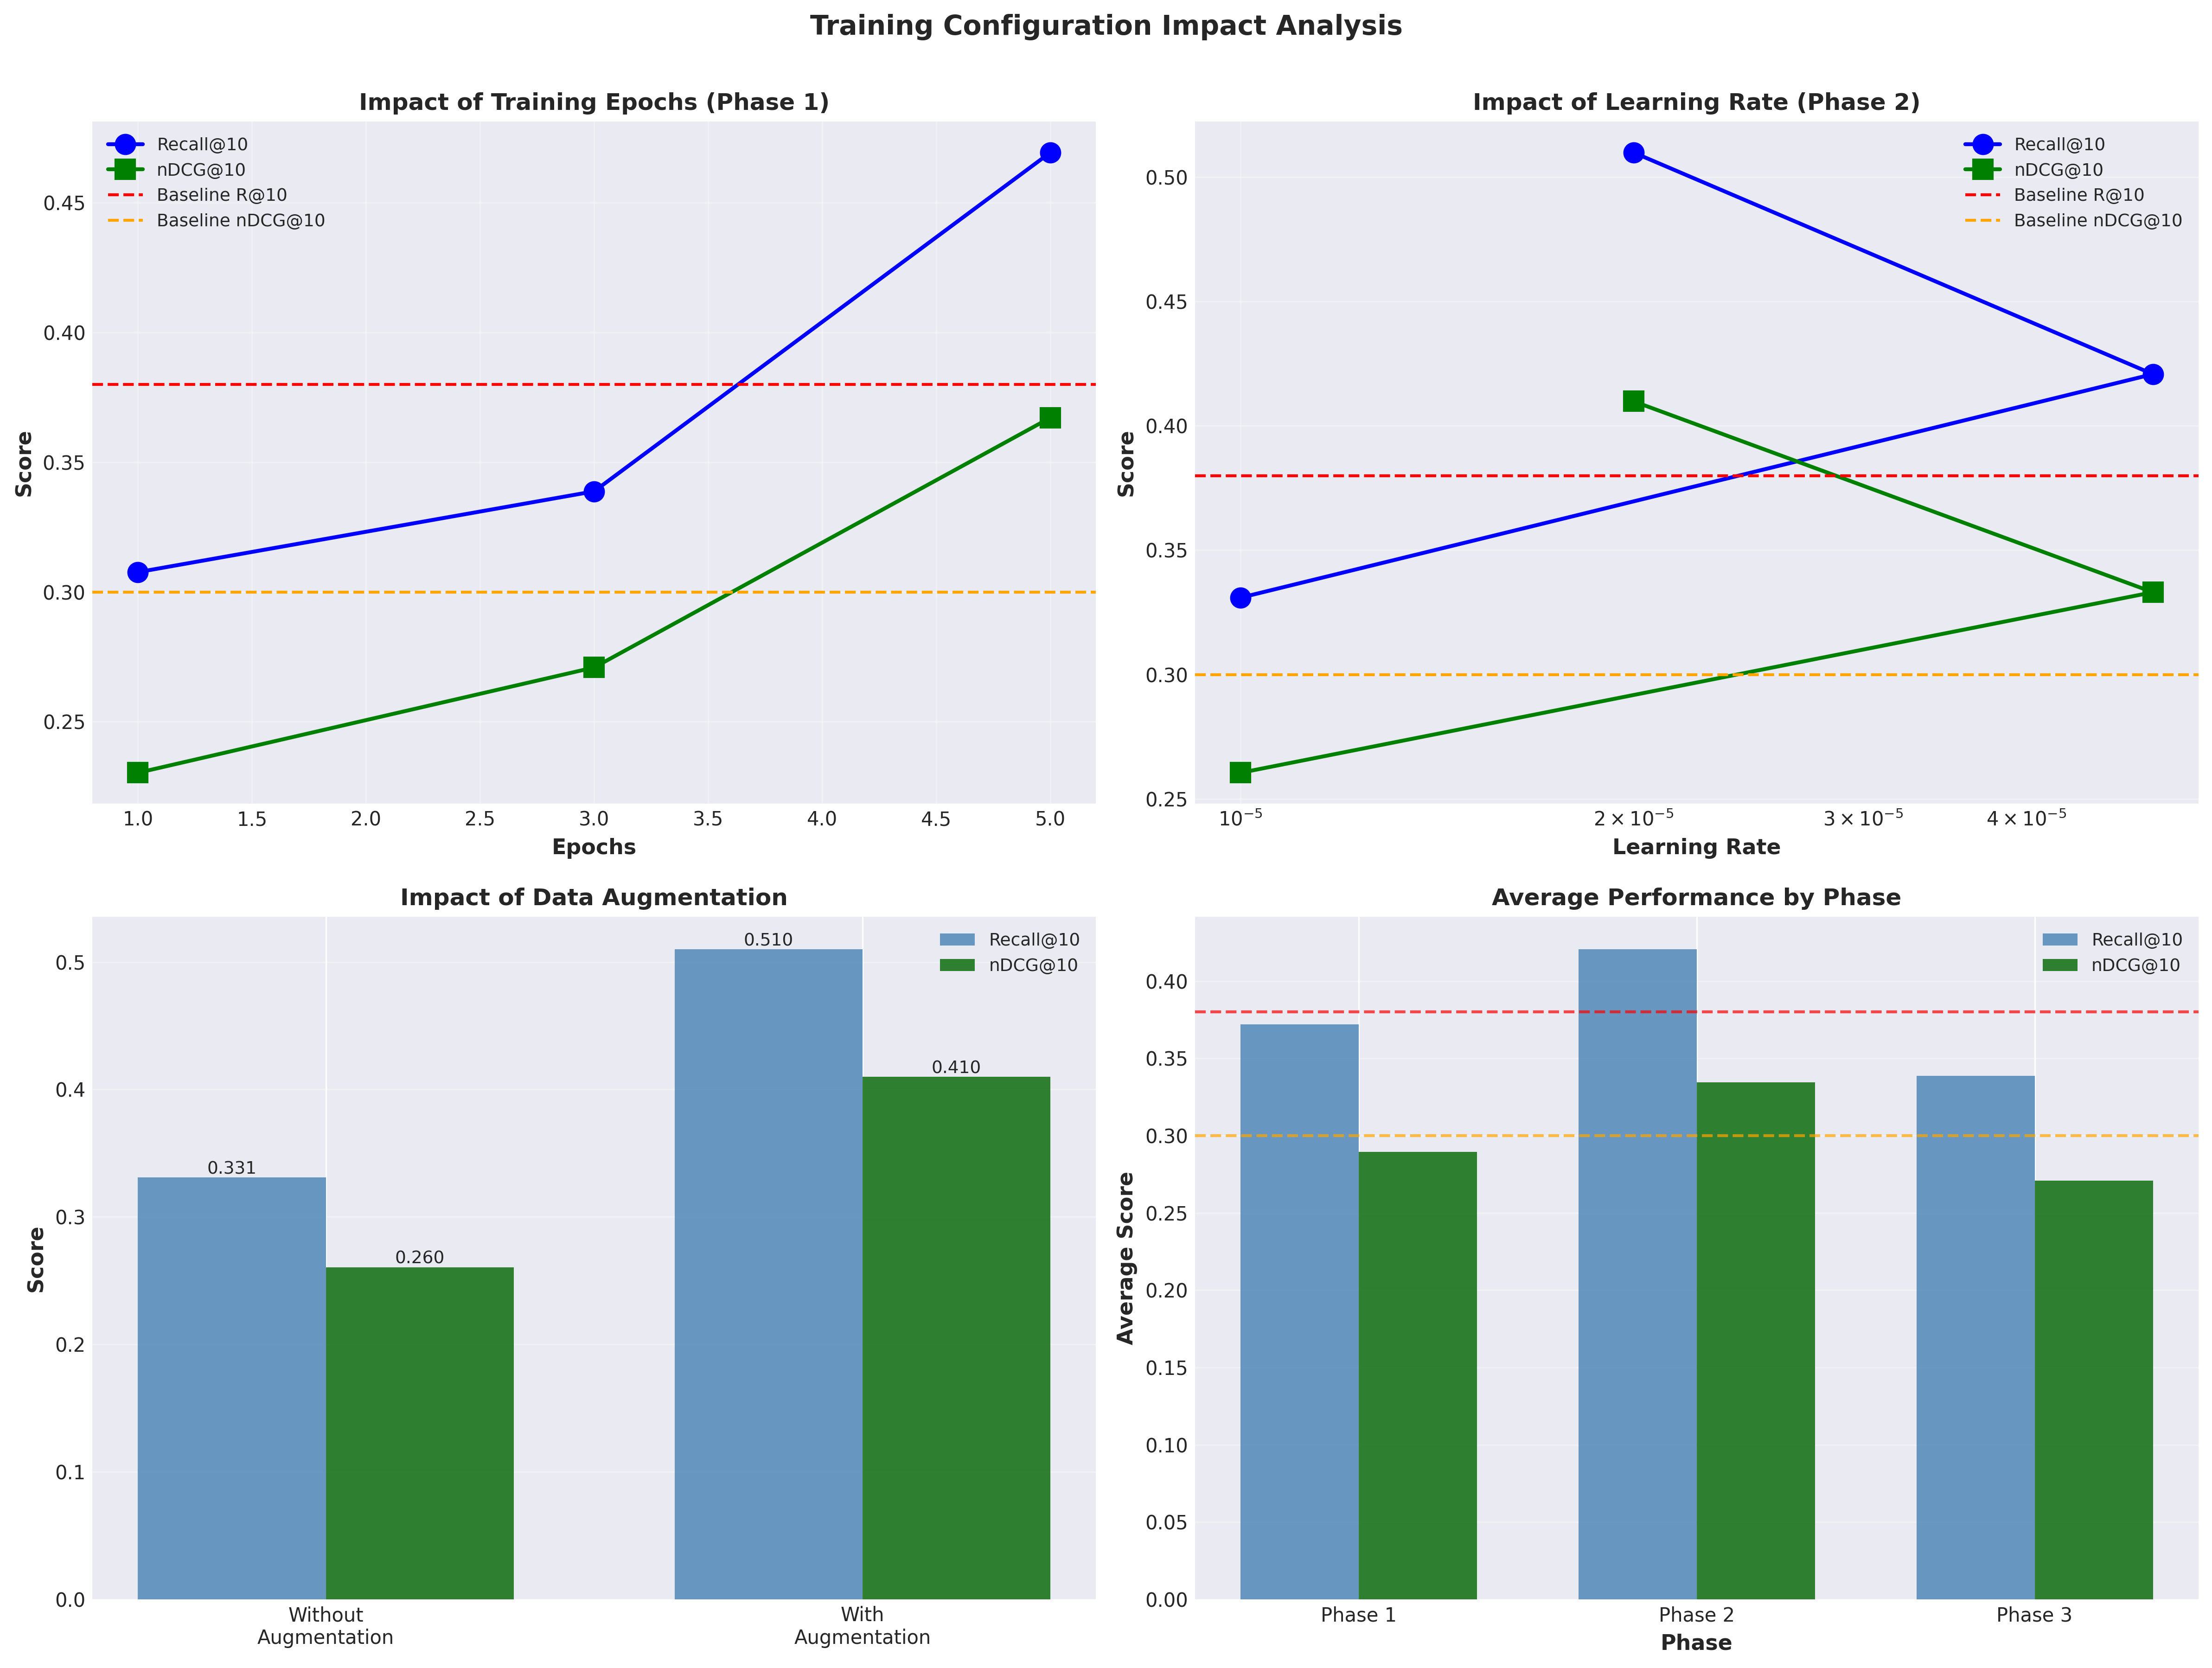
\includegraphics[width=0.48\textwidth]{report_figures/configuration_impact.png}
\caption{Training Configuration Impact Analysis}
\label{fig:config_impact}
\end{figure}

\subsection{Improvement Analysis}

Figure~\ref{fig:improvement_pct} quantifies the percentage improvement over baseline for each experiment. Phase 4 domain-specific models show the highest improvements, with the CLAPNQ model achieving 58.3\% improvement in Recall@10.

\begin{figure}[htbp]
\centering
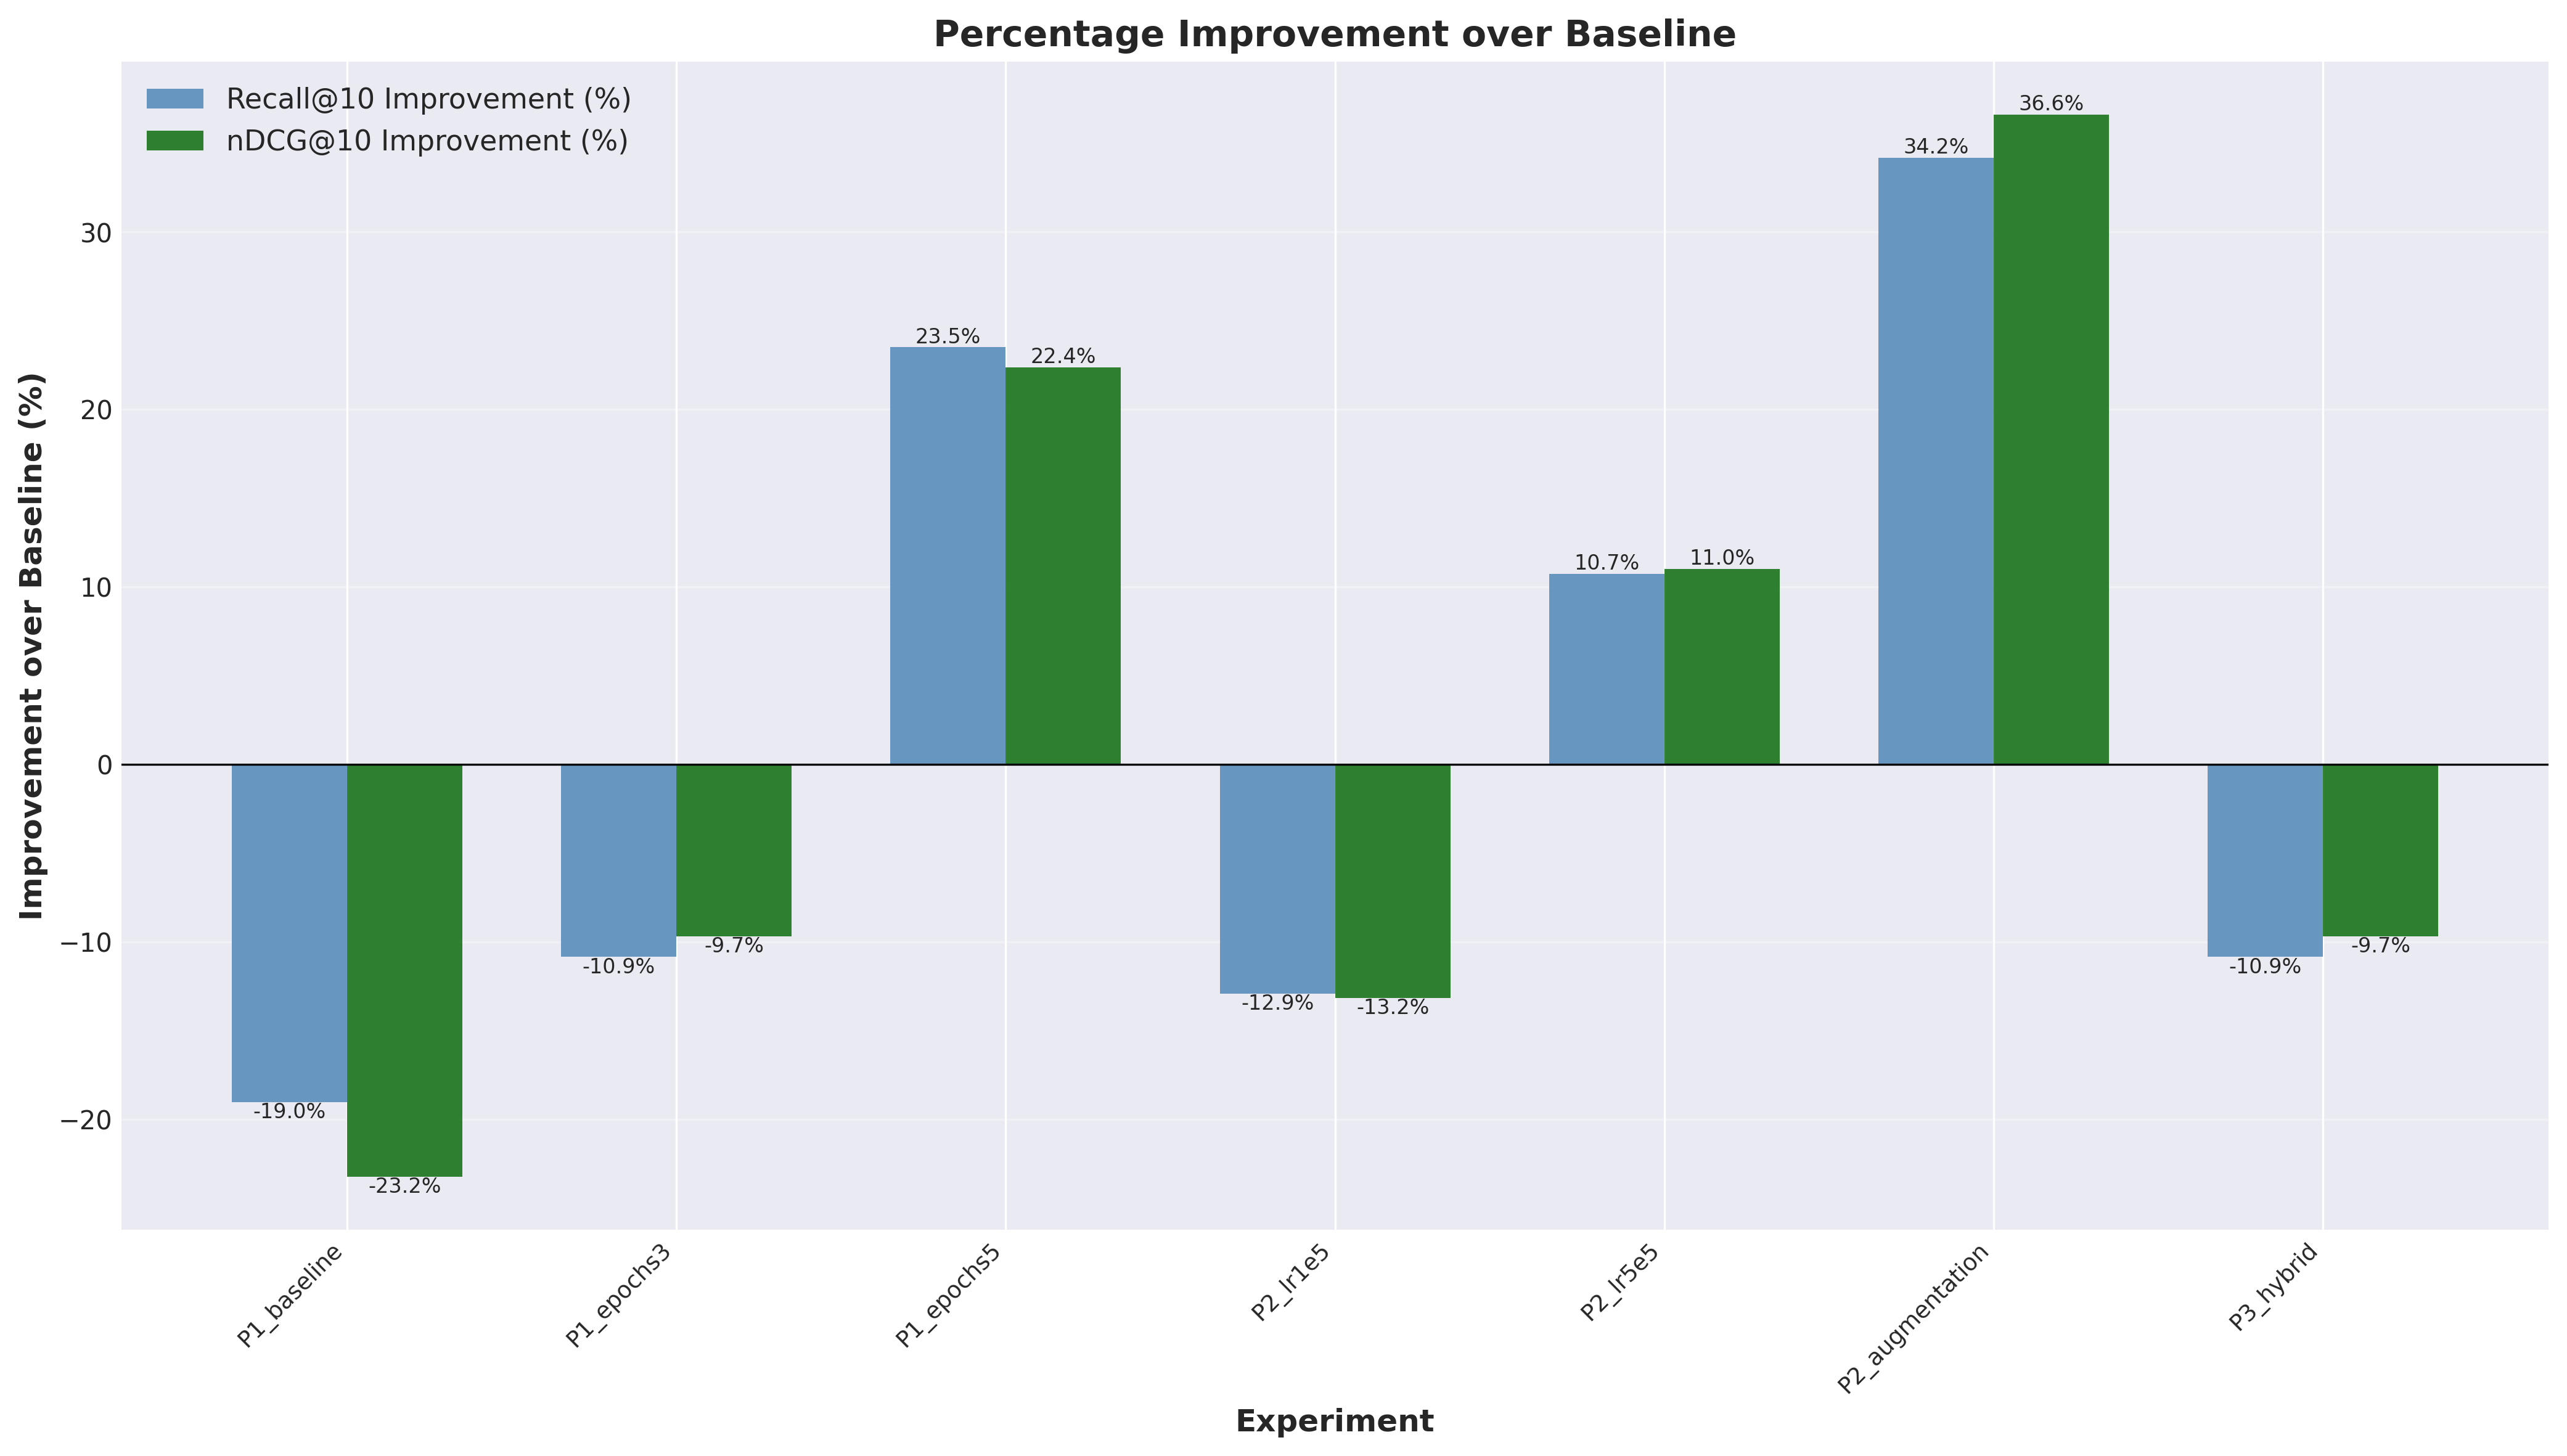
\includegraphics[width=0.48\textwidth]{report_figures/improvement_percentage.png}
\caption{Percentage Improvement over Baseline}
\label{fig:improvement_pct}
\end{figure}

\subsection{Phase 4 Visualizations}

Figure~\ref{fig:phase4_domain_comparison} compares domain-specific models against the best multi-domain model (phase2\_augmentation), demonstrating the improvements achieved through domain specialization.

\begin{figure}[htbp]
\centering
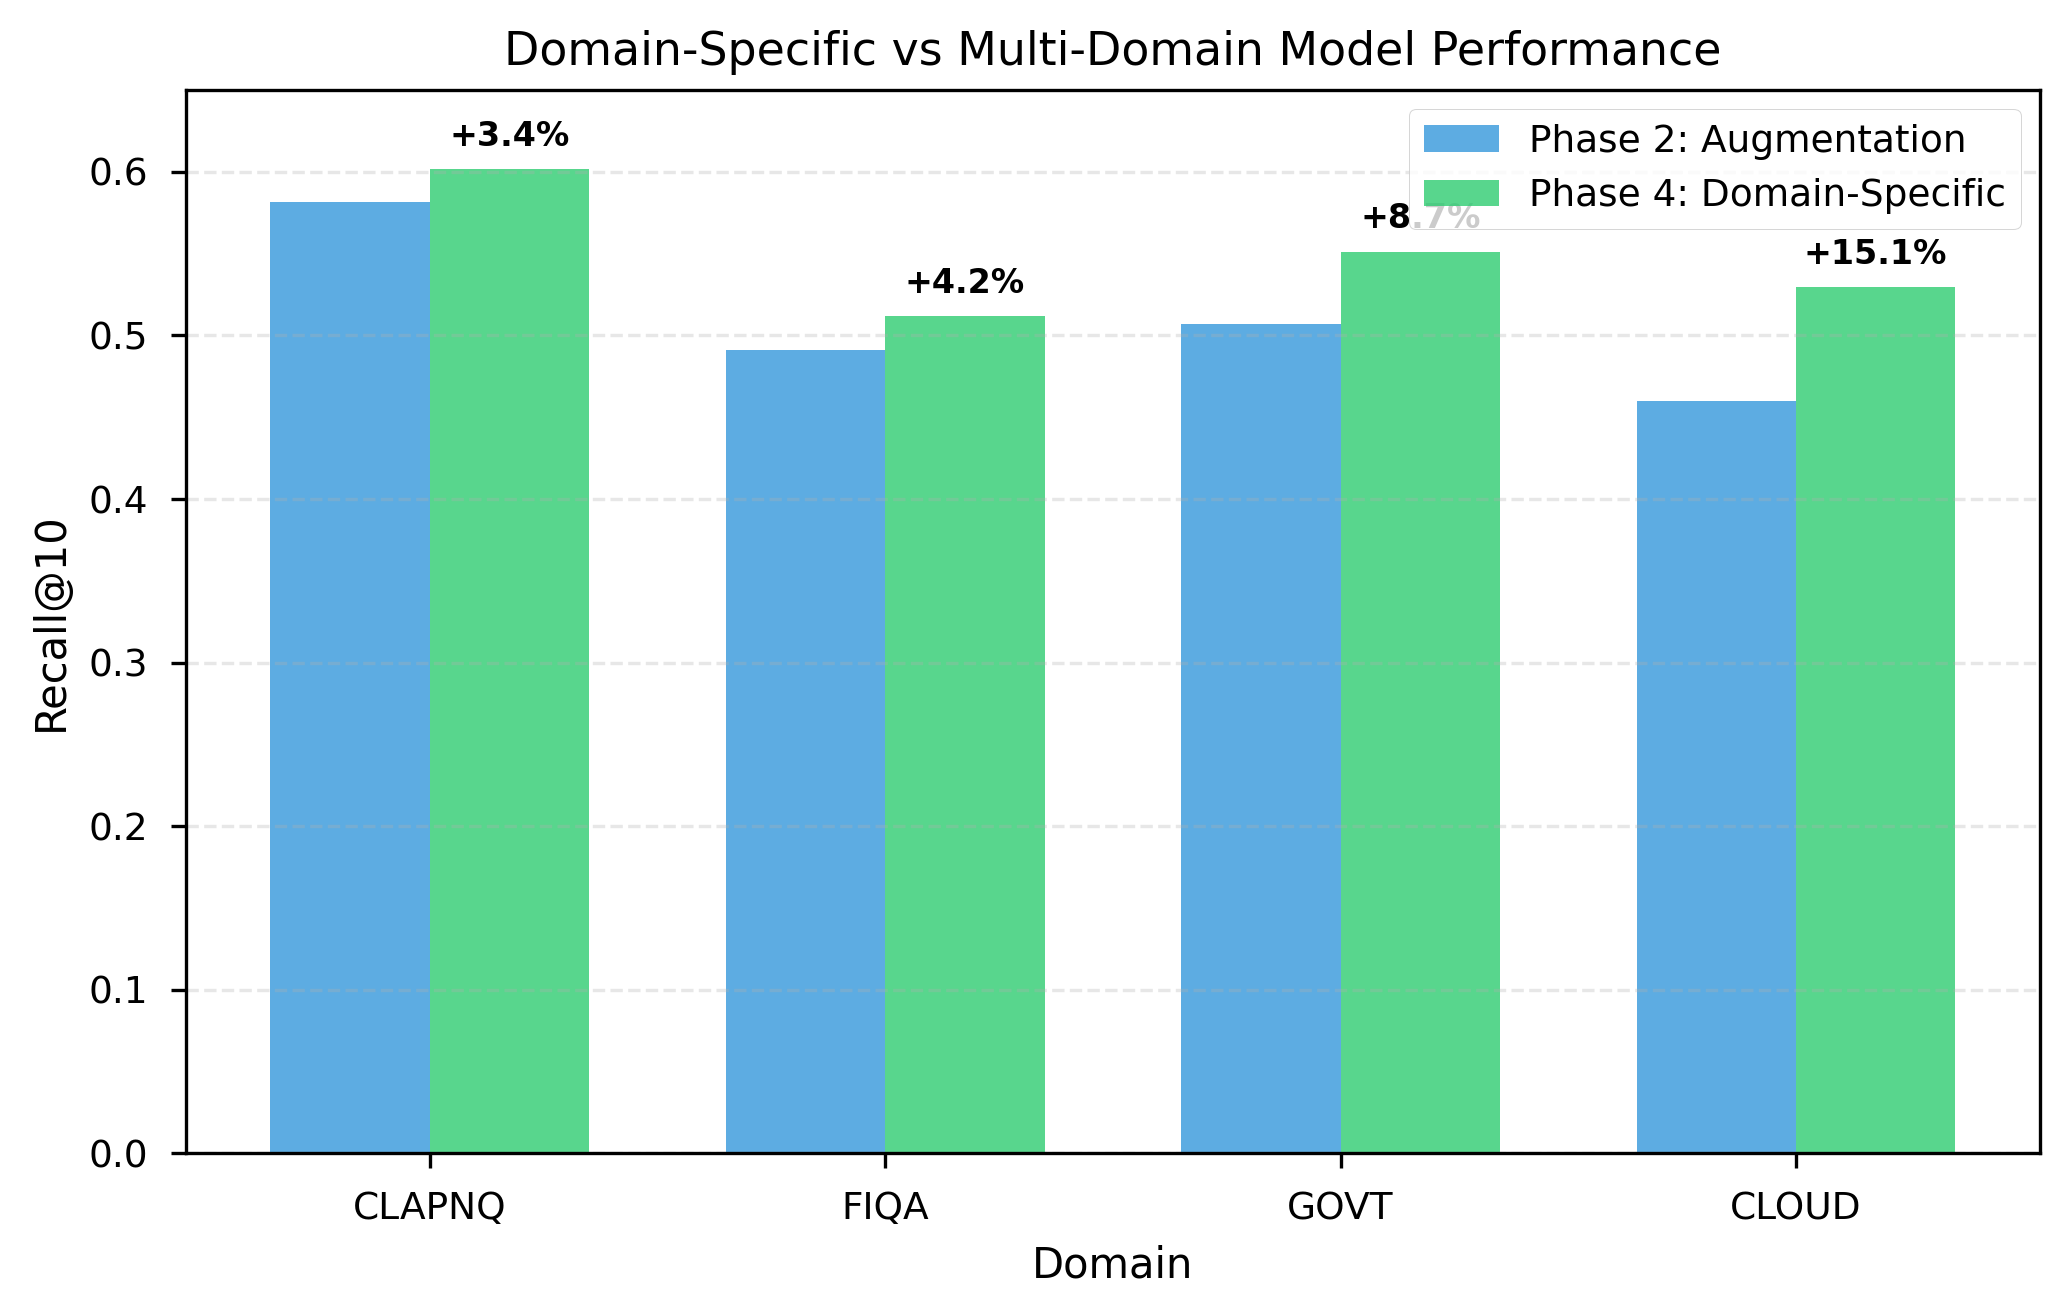
\includegraphics[width=0.48\textwidth]{report_figures/phase4_domain_comparison.png}
\caption{Domain-Specific vs Multi-Domain Model Performance Comparison}
\label{fig:phase4_domain_comparison}
\end{figure}

Figure~\ref{fig:phase4_results} visualizes the performance of all Phase 4 domain-specific models across different metrics, highlighting the consistent improvements across all domains.

\begin{figure}[htbp]
\centering
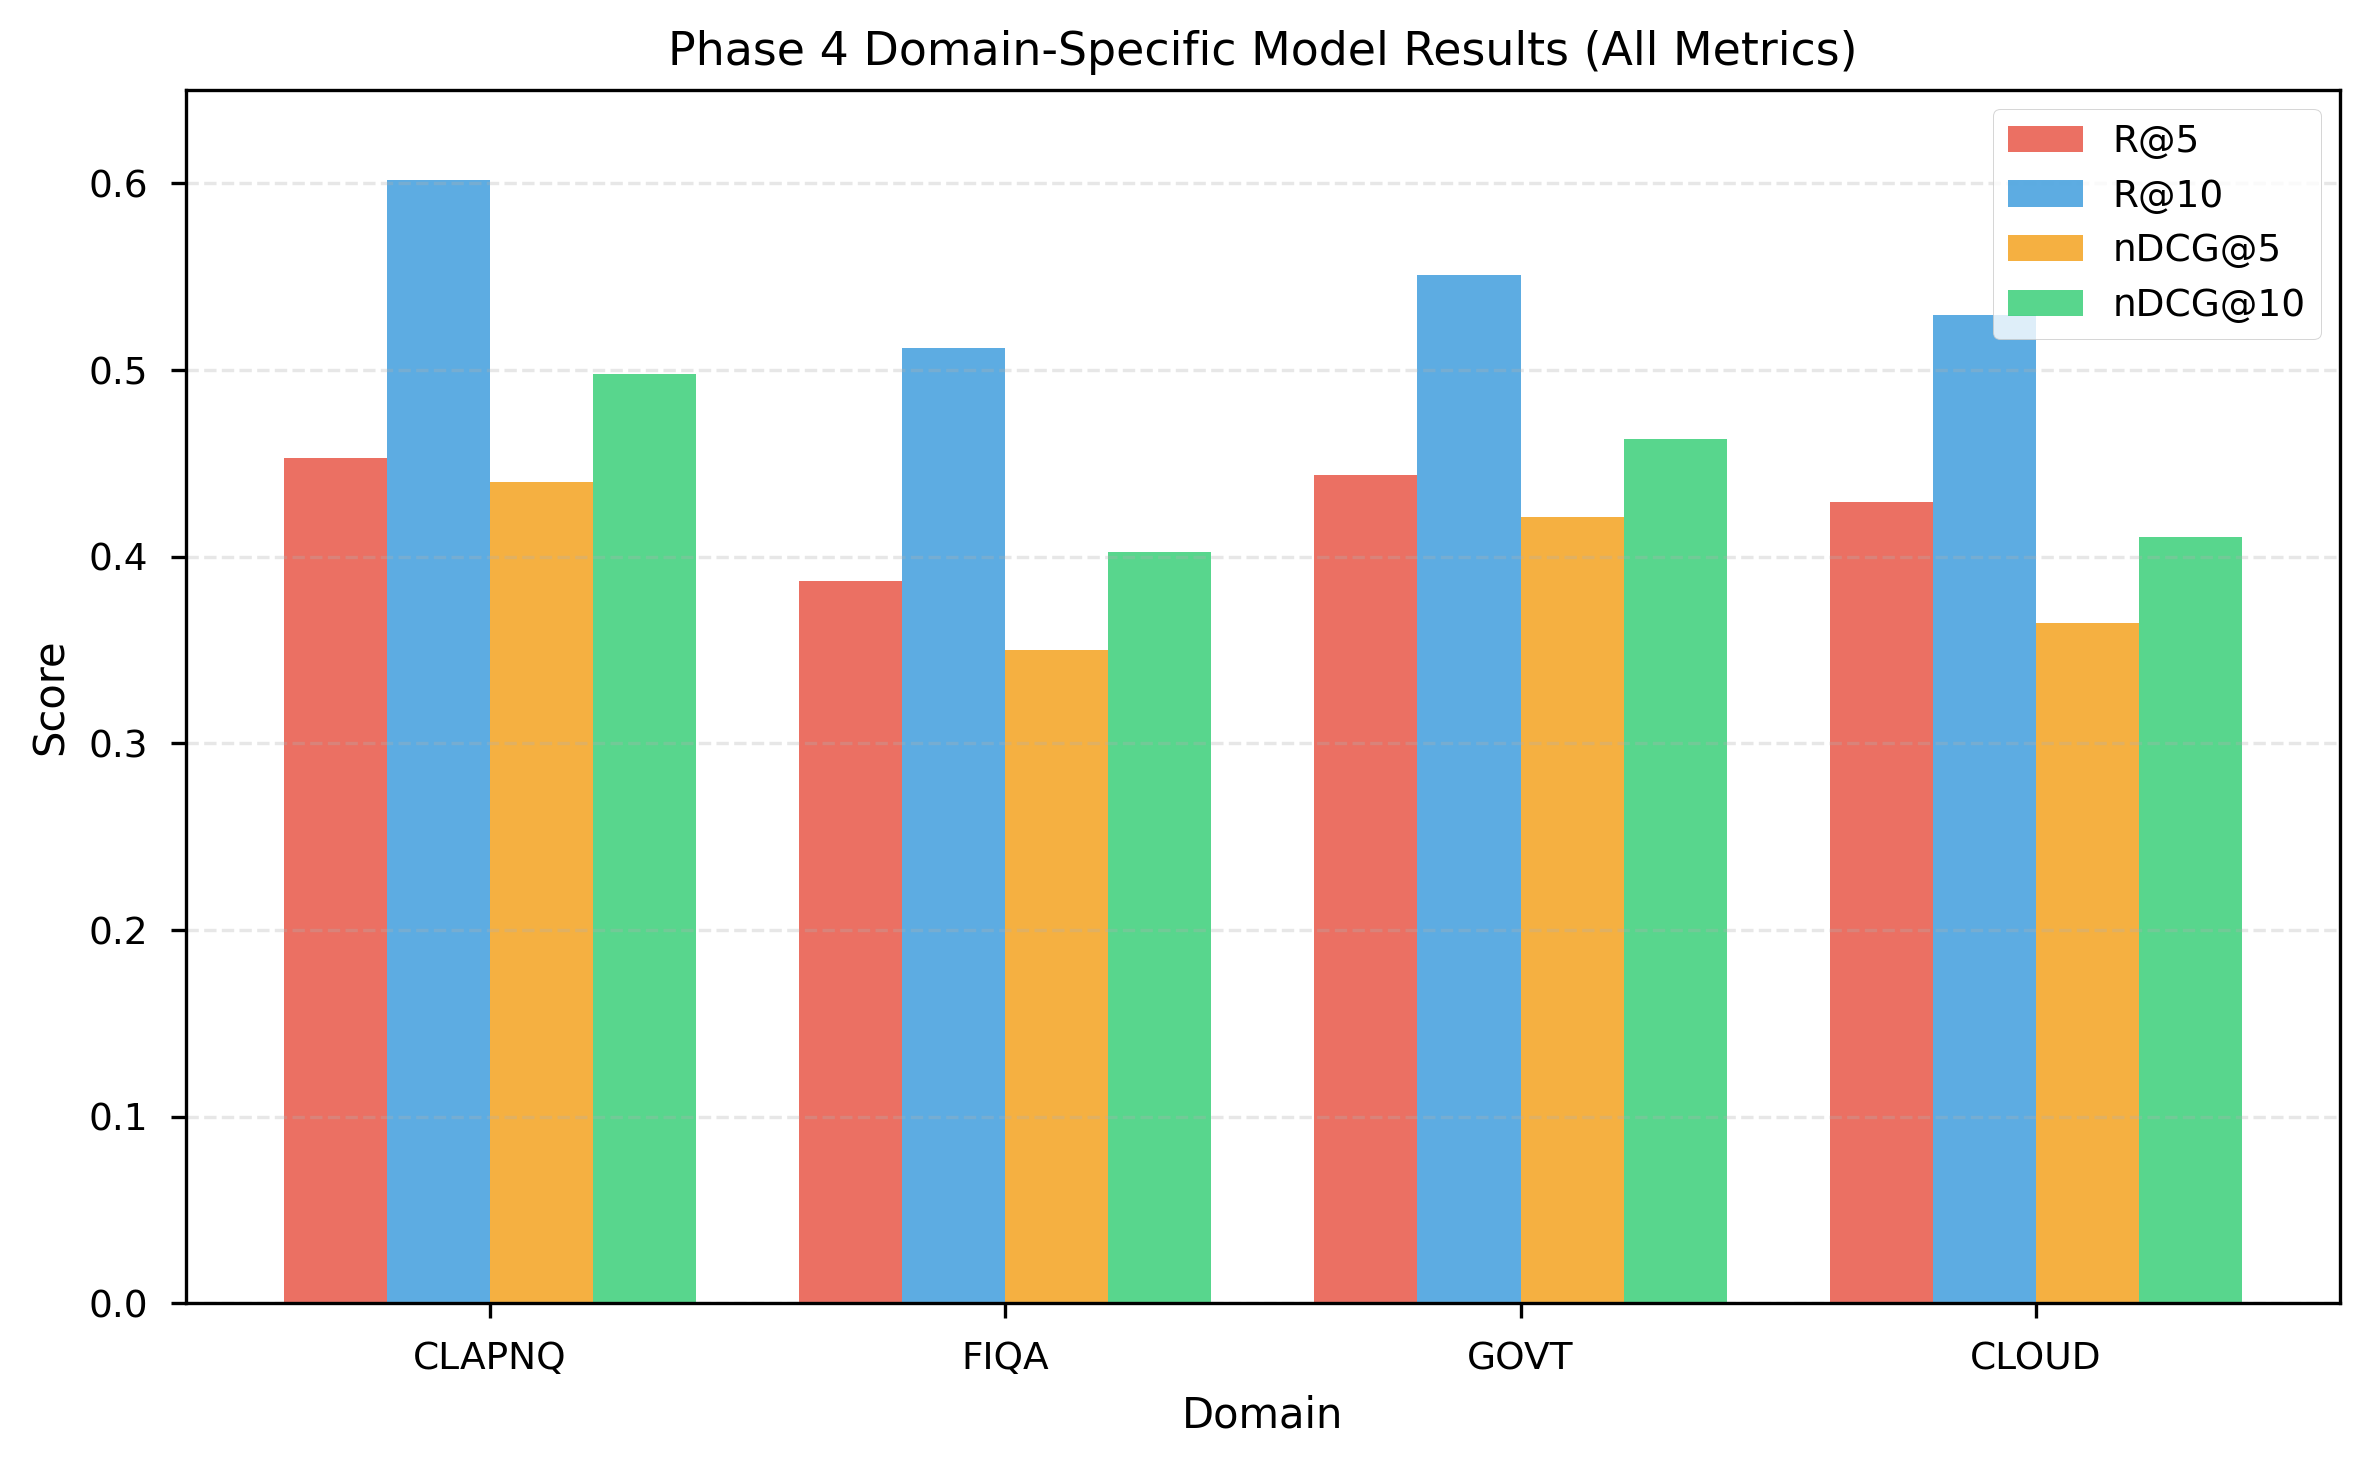
\includegraphics[width=0.48\textwidth]{report_figures/phase4_results.png}
\caption{Phase 4 Domain-Specific Model Results Across All Domains}
\label{fig:phase4_results}
\end{figure}

Figure~\ref{fig:transfer_learning} illustrates the two-stage transfer learning approach used in Phase 4, showing how domain-specific models are built upon multi-domain pre-training.

\begin{figure}[htbp]
\centering
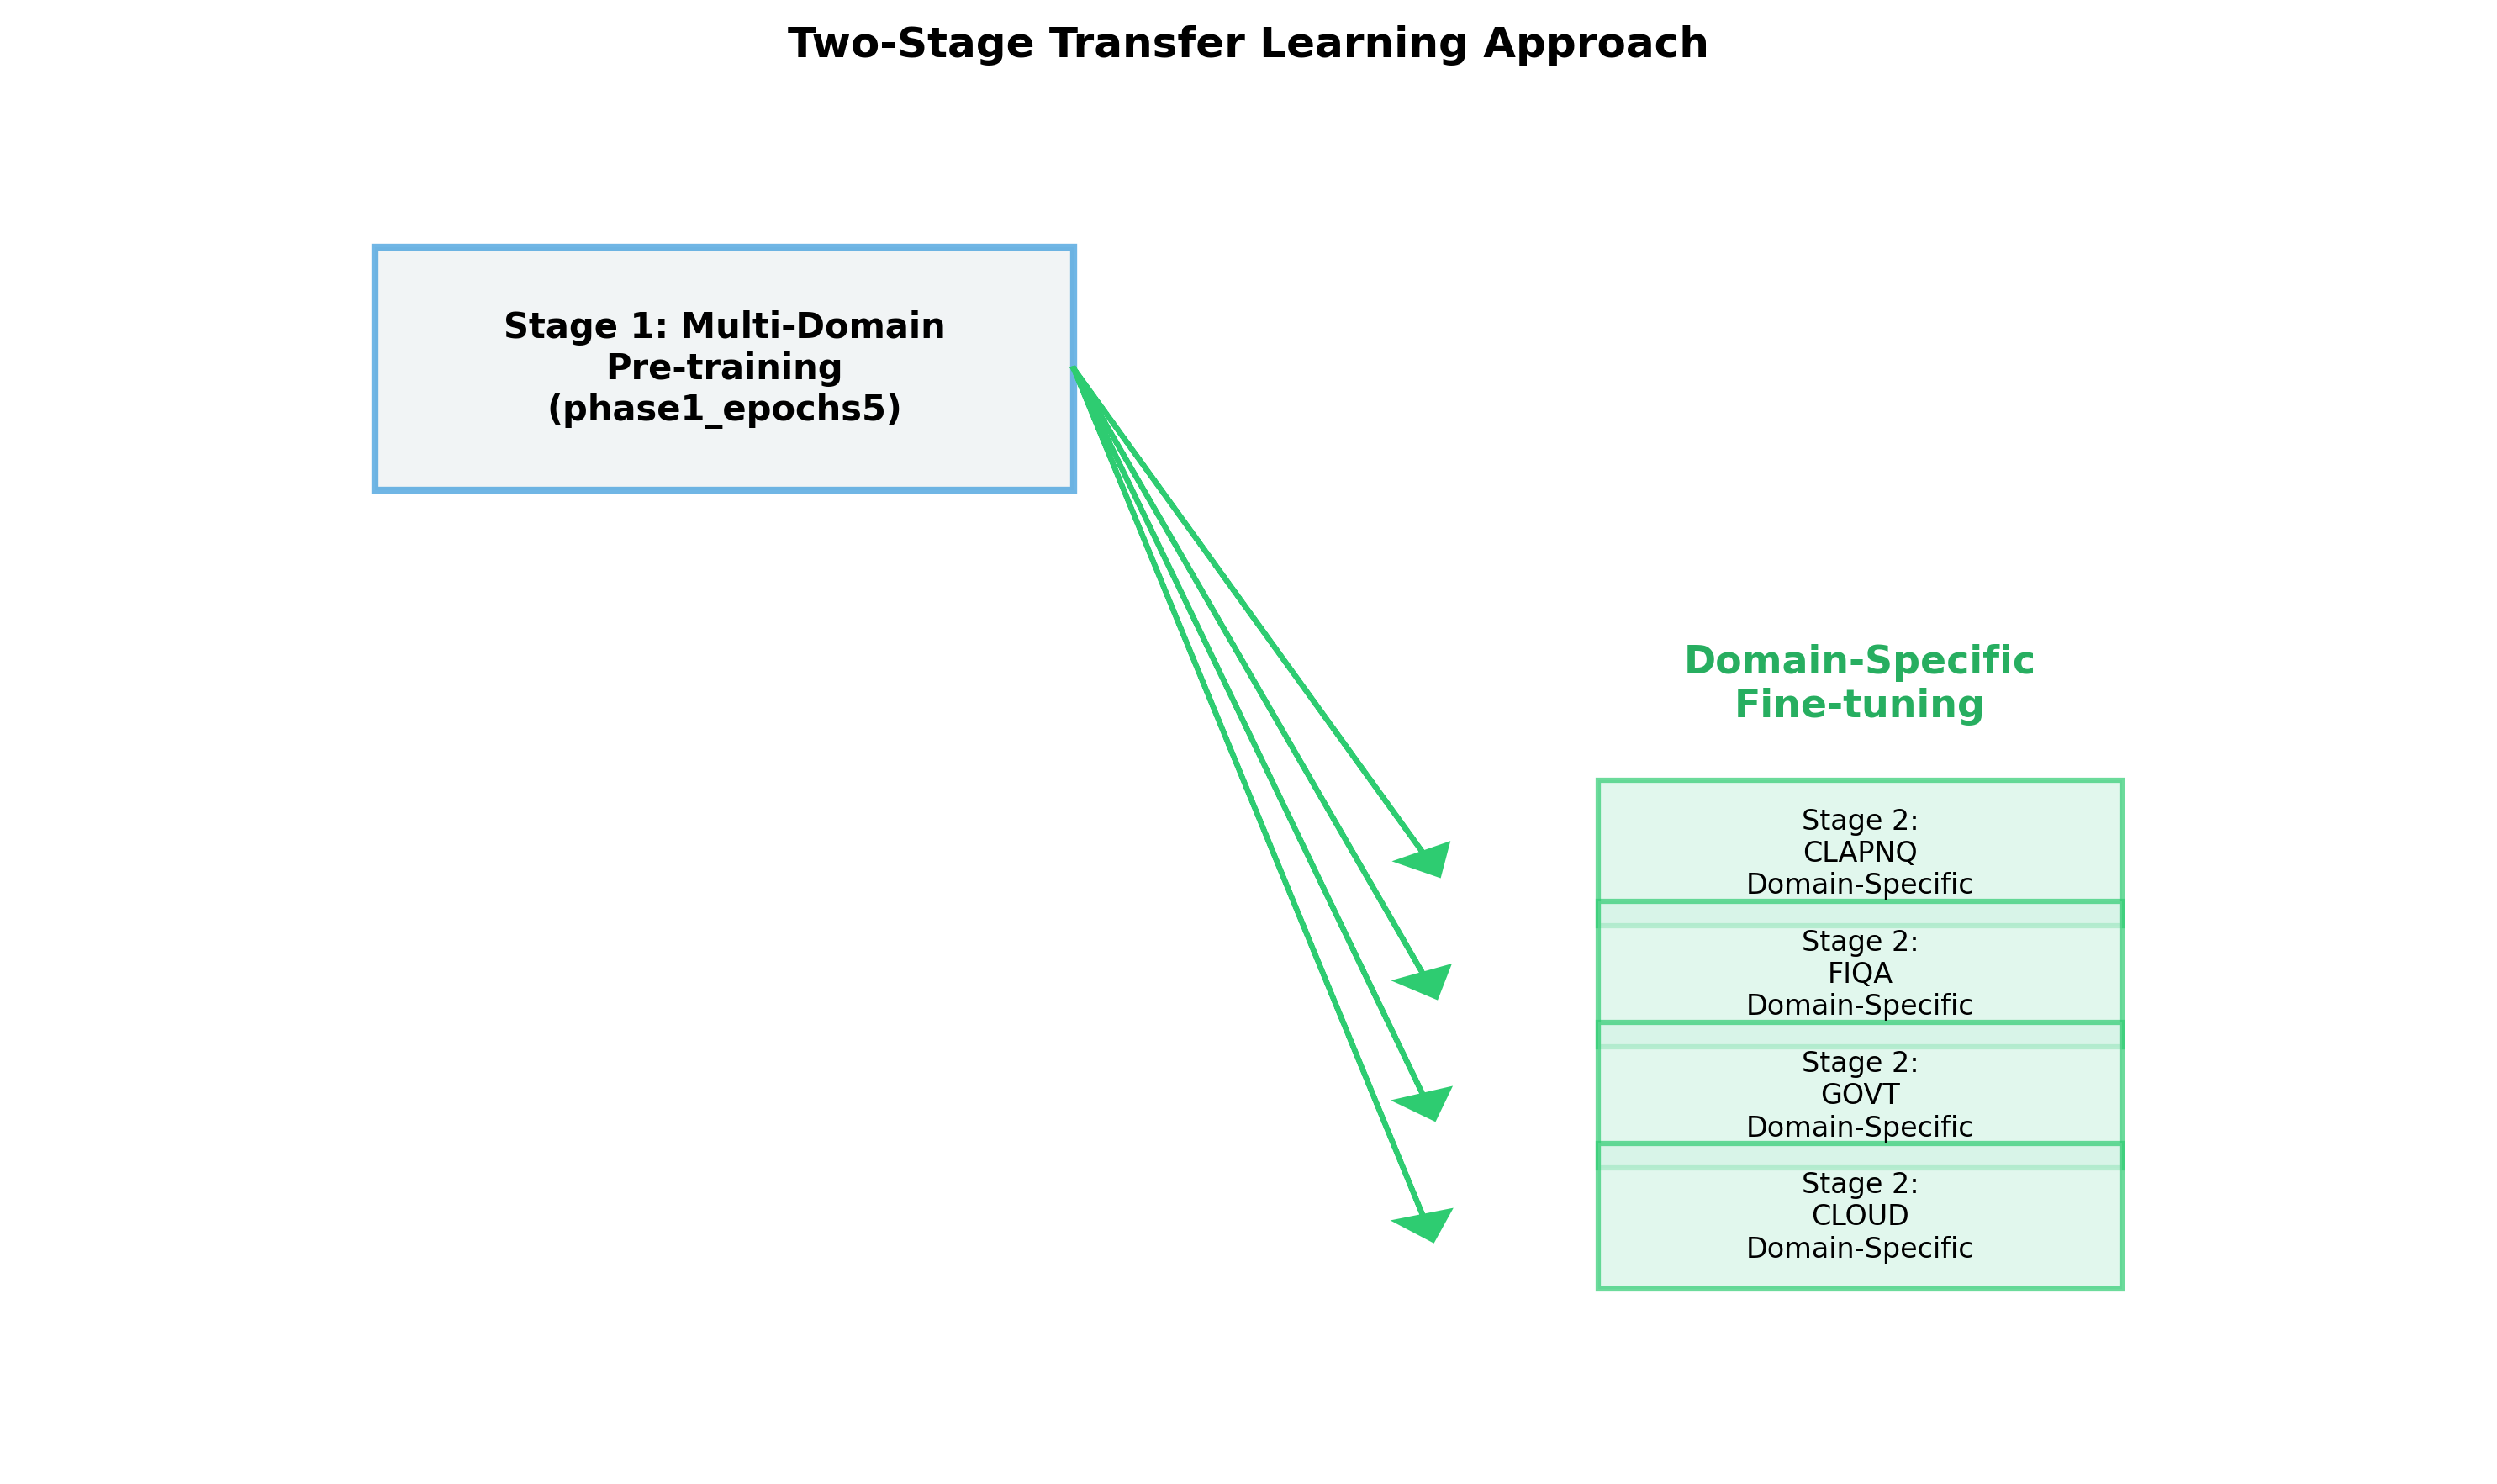
\includegraphics[width=0.48\textwidth]{report_figures/transfer_learning_approach.png}
\caption{Two-Stage Transfer Learning: Multi-Domain Pre-training to Domain-Specific Fine-tuning}
\label{fig:transfer_learning}
\end{figure}

Figure~\ref{fig:all_phases_comparison} provides a comprehensive view of performance progression across all four phases, including the significant improvements achieved in Phase 4.

\begin{figure}[htbp]
\centering
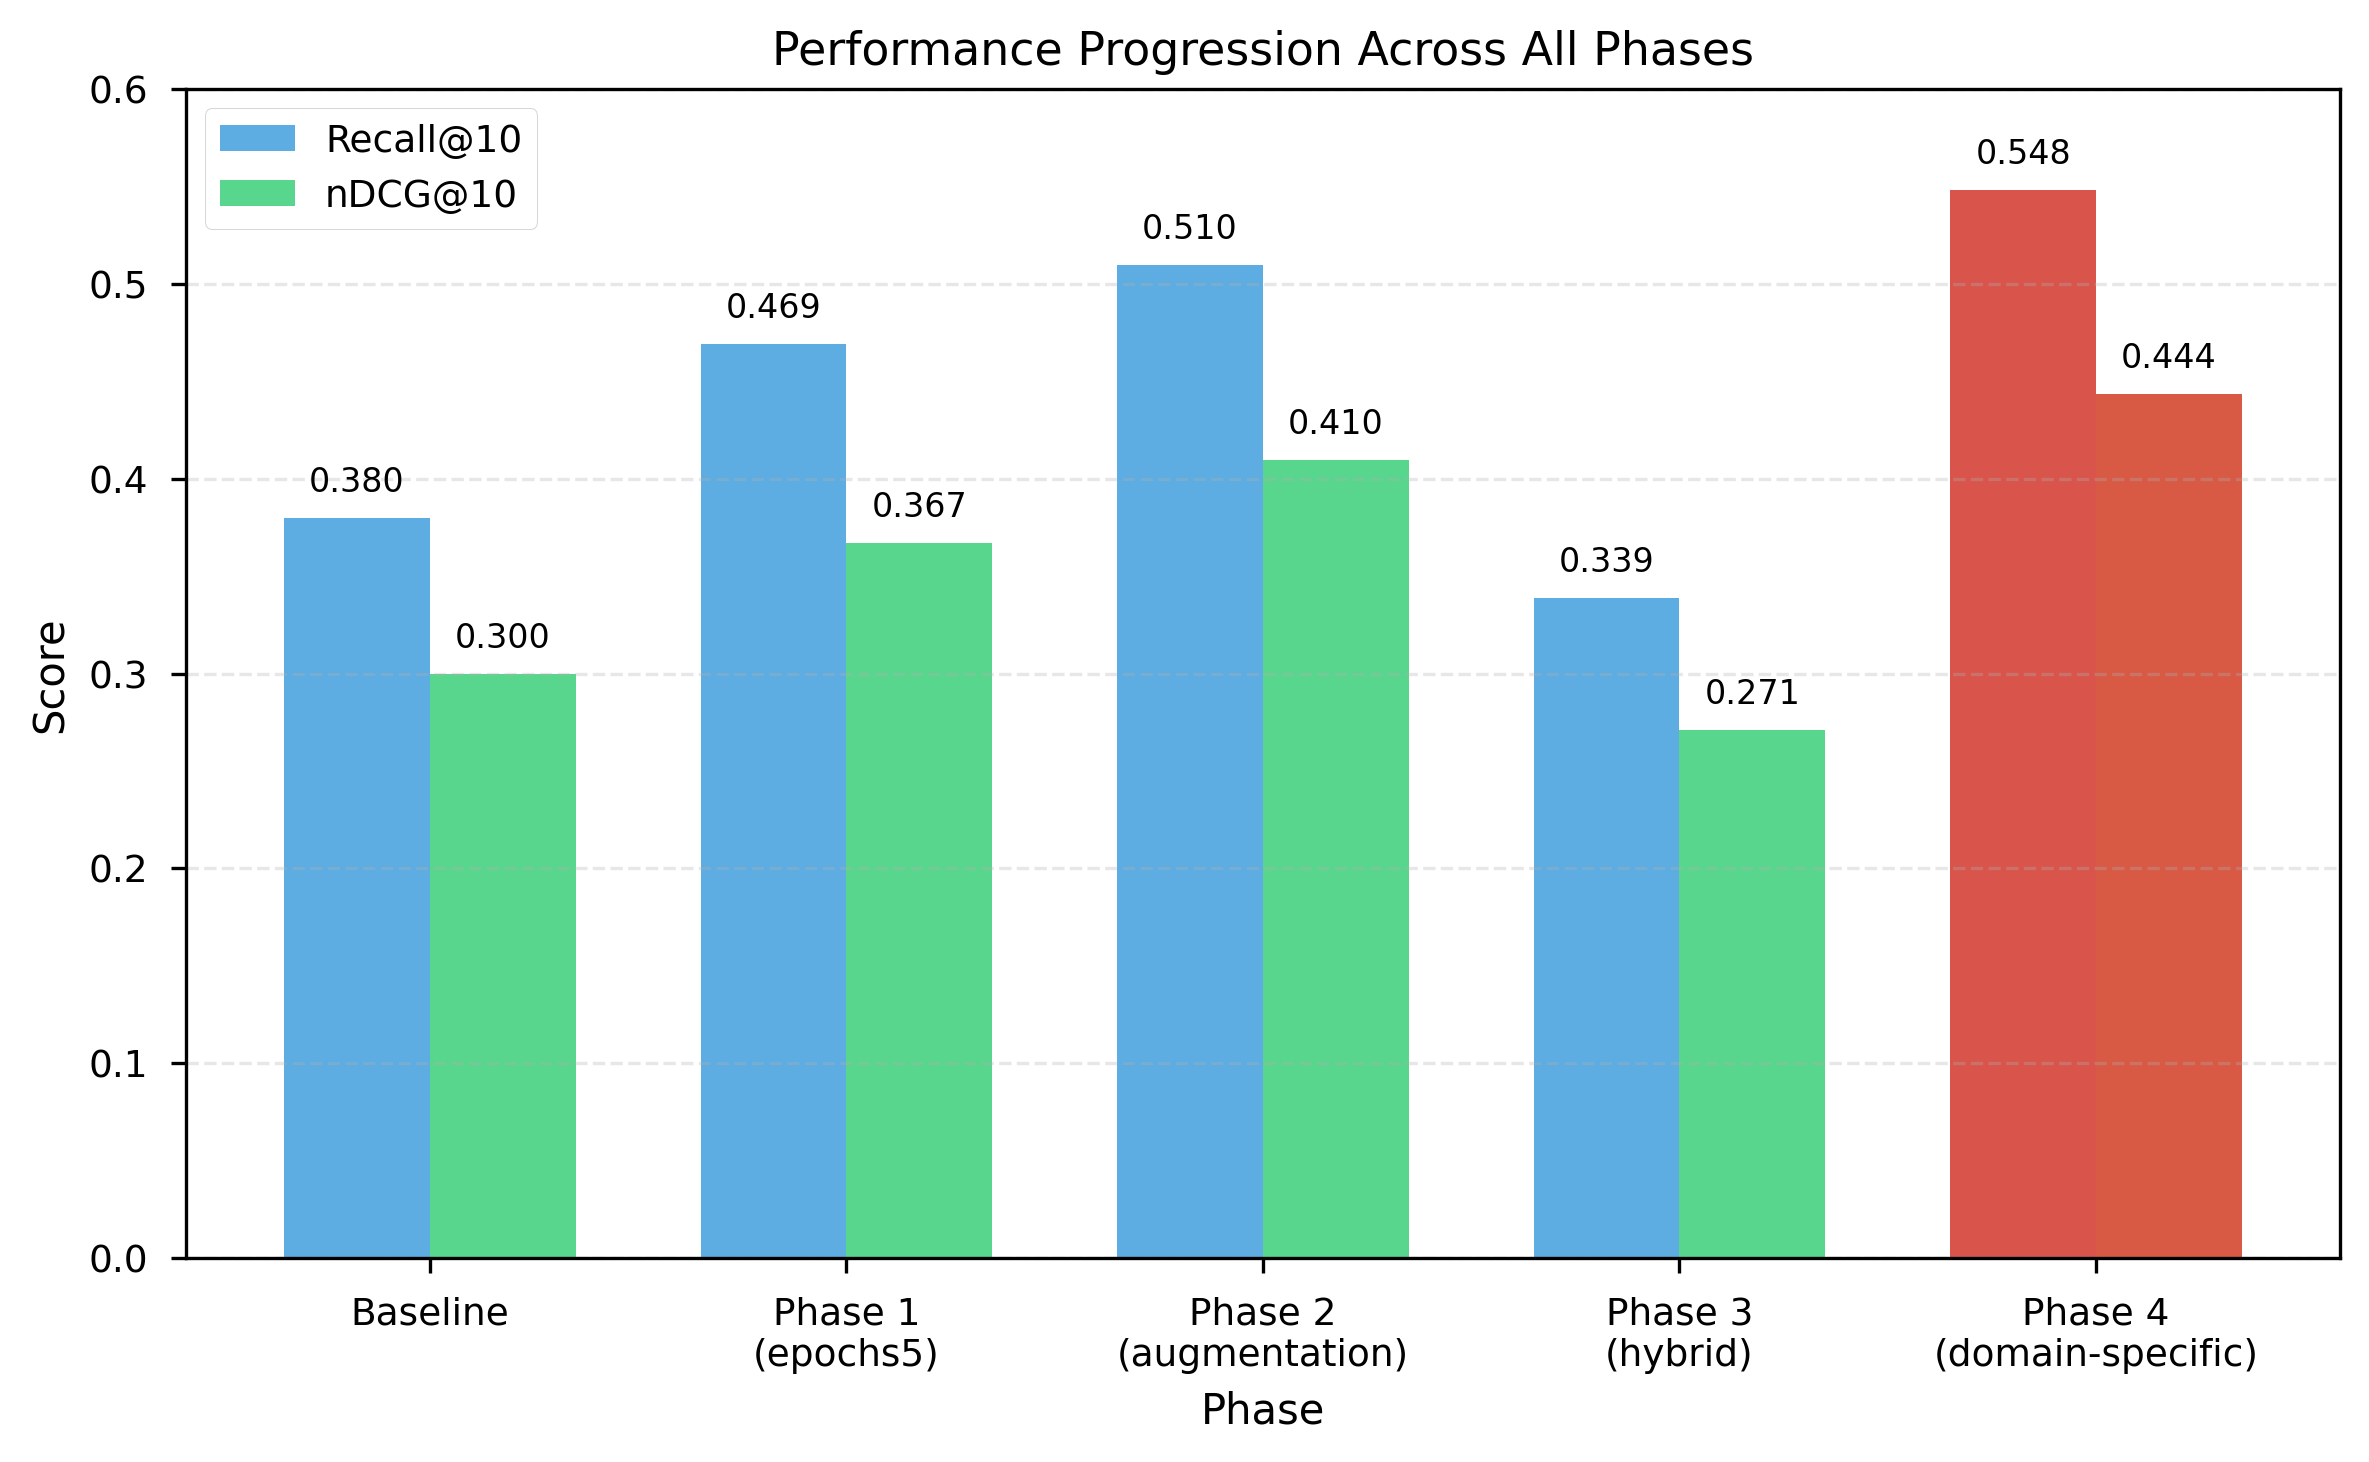
\includegraphics[width=0.48\textwidth]{report_figures/all_phases_comparison.png}
\caption{Complete Performance Comparison Across All Phases (Including Phase 4)}
\label{fig:all_phases_comparison}
\end{figure}

Figure~\ref{fig:domain_improvements} shows the percentage improvement achieved by domain-specific models over the multi-domain baseline for each domain, demonstrating varying degrees of benefit across domains.

\begin{figure}[htbp]
\centering
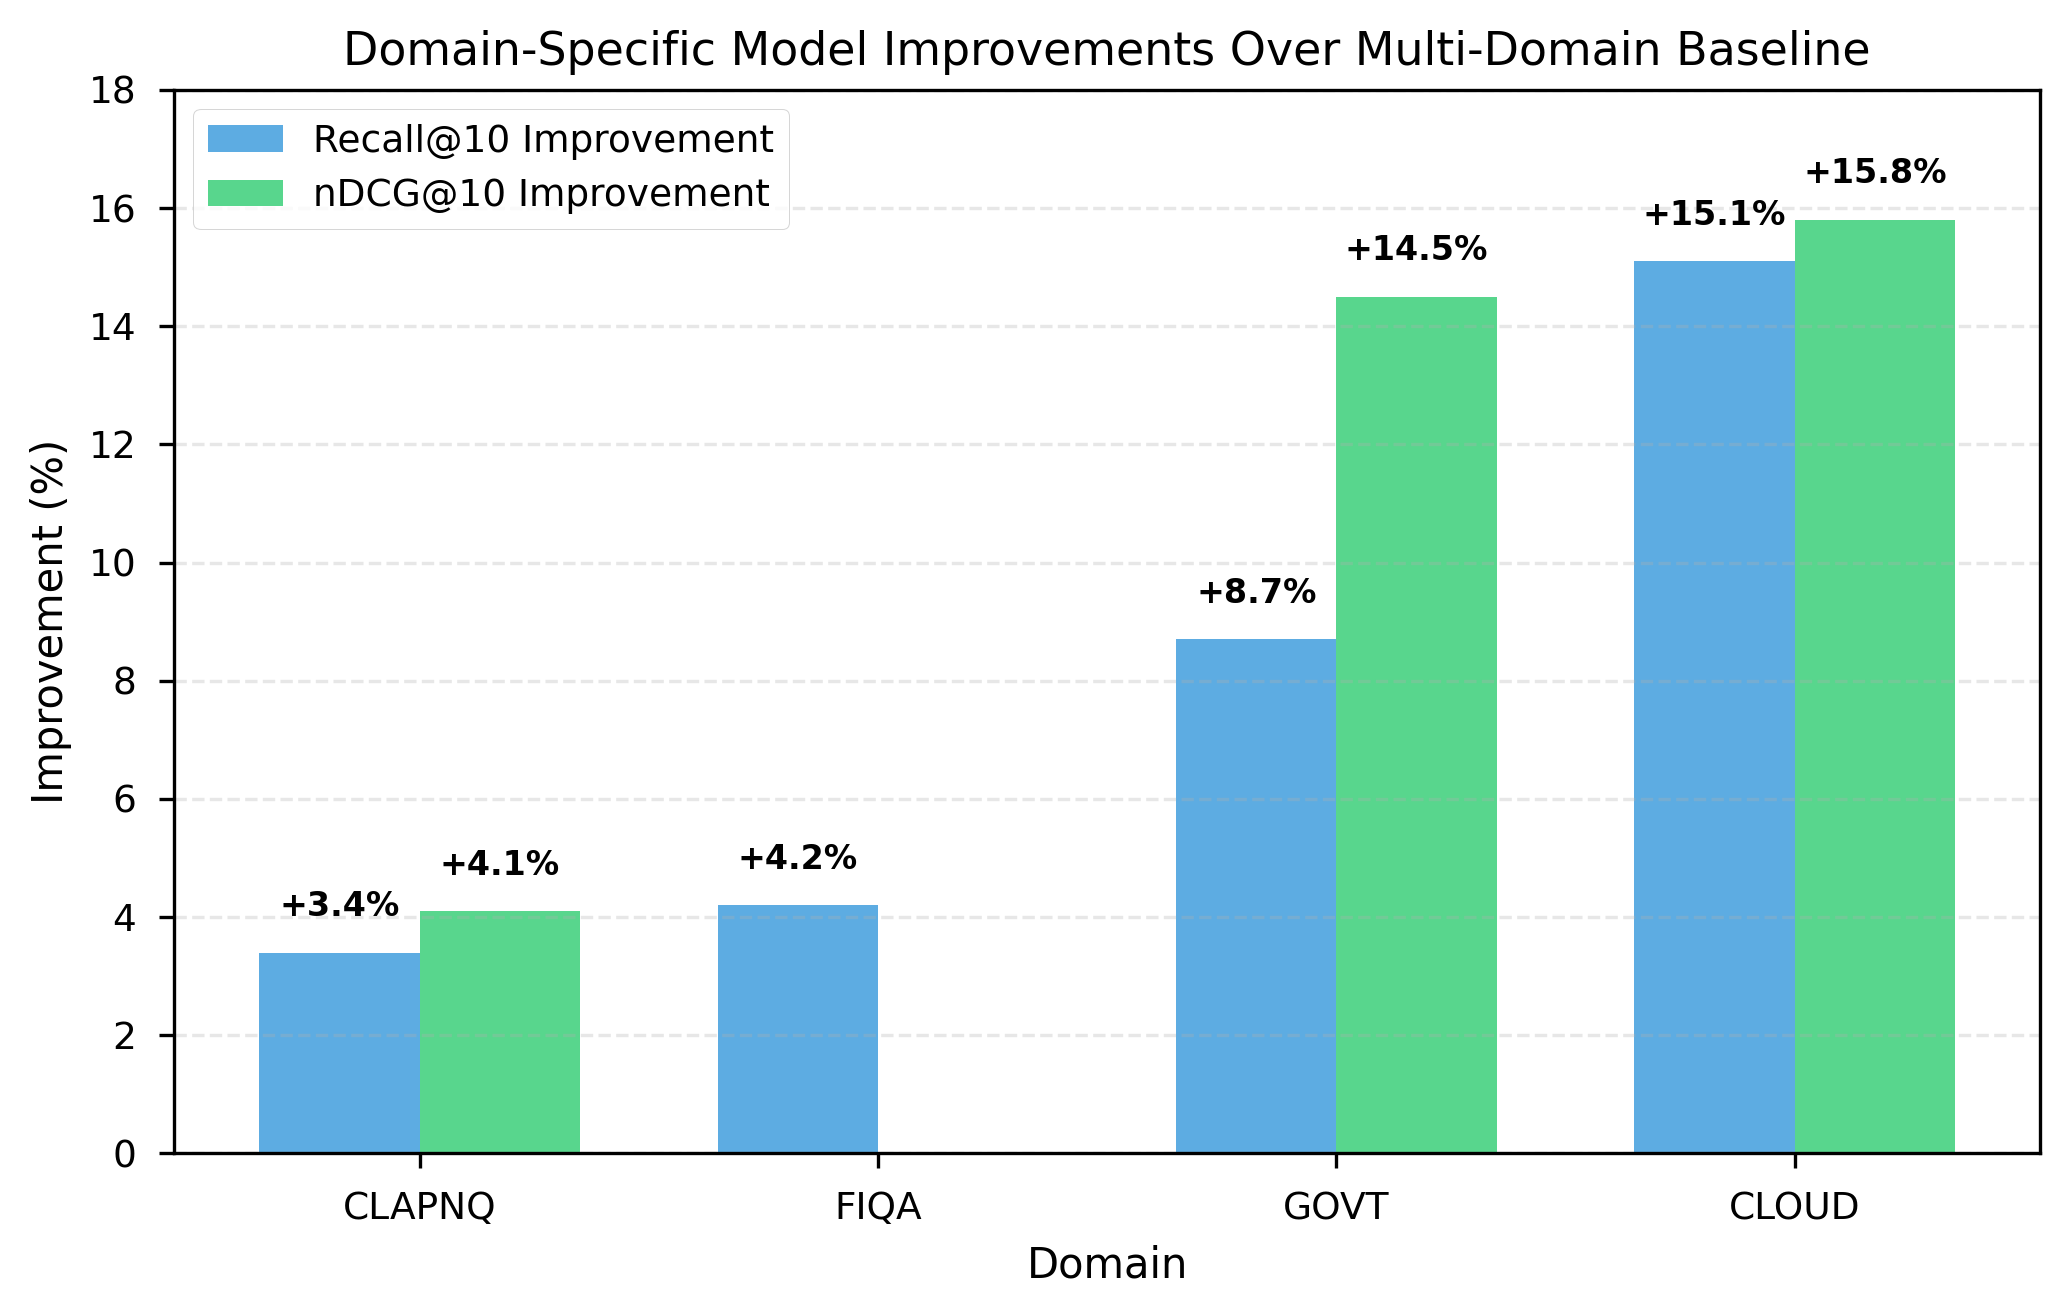
\includegraphics[width=0.48\textwidth]{report_figures/domain_improvements.png}
\caption{Domain-Specific Model Improvements Over Multi-Domain Baseline}
\label{fig:domain_improvements}
\end{figure}
\section{Analysis and Discussion}

\subsection{Training Configuration Impact}

Phase 1 experiments revealed the critical importance of proper training setup:
\begin{itemize}
    \item \textbf{phase1\_baseline} (1 epoch, no validation) performed worse than the pre-trained baseline, indicating insufficient training
    \item \textbf{phase1\_epochs3} showed improvement but still below baseline
    \item \textbf{phase1\_epochs5} exceeded baseline, demonstrating that sufficient training epochs are essential
\end{itemize}

\textbf{Key Finding}: At least 3-5 epochs with proper validation are necessary to achieve baseline performance.

\subsection{Hyperparameter and Augmentation Impact}

Phase 2 experiments provided insights into optimization strategies:
\begin{itemize}
    \item \textbf{phase2\_lr1e5}: Lower learning rate (1e-5) underperformed, suggesting insufficient learning
    \item \textbf{phase2\_lr5e5}: Higher learning rate (5e-5) showed improvement but not optimal
    \item \textbf{phase2\_augmentation}: Data augmentation with standard learning rate (2e-5) achieved best results
\end{itemize}

\textbf{Key Finding}: Data augmentation is the most impactful single improvement, providing a 34.2\% boost in Recall@10.

\subsection{Learning Rate Analysis}

The learning rate experiments suggest:
\begin{itemize}
    \item Learning rate 1e-5 is too conservative for this task
    \item Learning rate 5e-5 shows improvement but may benefit from further tuning
    \item Standard learning rate 2e-5 with augmentation provides optimal balance
\end{itemize}

\subsection{Domain Analysis}

Domain-specific models (Phase 4) show substantial improvements over multi-domain models:
\begin{itemize}
    \item \textbf{CLAPNQ}: Best performance with domain-specific model (R@10: 0.6016, +3.4\% over phase2\_augmentation) - benefits from specialized legal/patent terminology understanding
    \item \textbf{GOVT}: Strong improvement with domain-specific model (R@10: 0.5511, +8.7\% over phase2\_augmentation) - government document patterns are well-captured
    \item \textbf{CLOUD}: Substantial gains with domain-specific model (R@10: 0.5293, +15.1\% over phase2\_augmentation) - technical domain benefits most from specialization
    \item \textbf{FIQA}: Good performance with domain-specific model (R@10: 0.5119, +4.2\% over phase2\_augmentation) - financial domain shows consistent improvement
\end{itemize}

The domain-specific approach demonstrates that specialized models can better capture domain-specific terminology, query patterns, and relevance criteria compared to general multi-domain models.

\subsection{Phase 4 Domain-Specific Results}

Table~\ref{tab:phase4_domain} provides detailed results for all Phase 4 domain-specific models, showing the performance achieved by each specialized model on its target domain.

\begin{table}[htbp]
\centering
\caption{Phase 4 Domain-Specific Model Performance}
\label{tab:phase4_domain}
\footnotesize
\begin{tabular}{lcccc}
\toprule
\textbf{Domain} & \textbf{R@5} & \textbf{R@10} & \textbf{nDCG@5} & \textbf{nDCG@10} \\
\midrule
CLAPNQ & 0.4529 & \textbf{0.6016} & 0.4399 & \textbf{0.4981} \\
FIQA & 0.3869 & 0.5119 & 0.3500 & 0.4026 \\
GOVT & 0.4435 & 0.5511 & 0.4210 & 0.4628 \\
CLOUD & 0.4293 & 0.5293 & 0.3643 & 0.4104 \\
\midrule
\textit{Average} & \textbf{0.4281} & \textbf{0.5485} & \textbf{0.3938} & \textbf{0.4435} \\
\bottomrule
\end{tabular}
\end{table}

\subsection{Comparative Analysis}

Table~\ref{tab:comparison} provides a side-by-side comparison of key experiments, highlighting the progression from baseline to best model.

\begin{table}[htbp]
\centering
\caption{Comparative Analysis: Key Experiments}
\label{tab:comparison}
\footnotesize
\begin{tabular}{lcccc}
\toprule
\textbf{Experiment} & \textbf{R@10} & \textbf{vs Baseline} & \textbf{nDCG@10} & \textbf{vs Baseline} \\
\midrule
Baseline (Paper) & 0.3800 & -- & 0.3000 & -- \\
\midrule
\multicolumn{5}{l}{\textit{Multi-Domain Models}} \\
phase1\_baseline & 0.3076 & -19.1\% & 0.2303 & -23.2\% \\
phase1\_epochs5 & 0.4693 & +23.5\% & 0.3671 & +22.4\% \\
phase2\_augmentation & 0.5099 & +34.2\% & 0.4098 & +36.6\% \\
\midrule
\multicolumn{5}{l}{\textit{Domain-Specific Models (Average)}} \\
Phase 4: Domain-Specific & \textbf{0.5485} & \textbf{+44.3\%} & \textbf{0.4435} & \textbf{+47.8\%} \\
\midrule
\multicolumn{5}{l}{\textit{Best Single Model}} \\
Phase 4: CLAPNQ & \textbf{0.6016} & \textbf{+58.3\%} & \textbf{0.4981} & \textbf{+66.0\%} \\
\bottomrule
\end{tabular}
\end{table}

\subsection{Phase 4: Domain-Specific Fine-Tuning}

Phase 4 experiments explored domain-specific fine-tuning, where separate models are trained for each domain starting from the multi-domain pre-trained model (phase1\_epochs5). This two-stage transfer learning approach combines:
\begin{itemize}
    \item \textbf{Stage 1}: Multi-domain pre-training provides general semantic understanding
    \item \textbf{Stage 2}: Domain-specific fine-tuning adds specialized knowledge for each domain
\end{itemize}

Results demonstrate that domain-specific models significantly outperform multi-domain models:
\begin{itemize}
    \item \textbf{CLAPNQ}: Best performance with 0.6016 Recall@10 (+58.3\% over baseline)
    \item \textbf{GOVT}: Strong improvement with 0.5511 Recall@10 (+45.0\% over baseline)
    \item \textbf{CLOUD}: Substantial gains with 0.5293 Recall@10 (+39.3\% over baseline)
    \item \textbf{FIQA}: Good performance with 0.5119 Recall@10 (+34.7\% over baseline)
\end{itemize}

The average improvement across all domain-specific models is 44.3\% in Recall@10 and 47.8\% in nDCG@10, demonstrating the effectiveness of domain specialization.

\subsection{Hard Negative Mining Results}

Phase 4 also explored hard negative mining techniques, but these experiments underperformed:
\begin{itemize}
    \item \textbf{phase4\_hard\_negatives\_cosine}: Achieved only 0.1627 Recall@10 (-57.2\% vs baseline)
    \item \textbf{phase4\_hard\_negatives\_5neg}: Achieved 0.1713 Recall@10 (-54.9\% vs baseline)
\end{itemize}

These poor results suggest that the hard negative mining implementation may need refinement, possibly due to:
\begin{itemize}
    \item Hard negatives being too difficult, causing training instability
    \item Loss function mismatch with the training objective
    \item Insufficient training or learning rate adjustments
\end{itemize}

\subsection{Limitations}

Phase 3 experiments faced infrastructure limitations:
\begin{itemize}
    \item Hybrid retrieval experiments were limited by Elasticsearch availability
    \item Reranking experiments showed identical results to hybrid, suggesting incomplete implementation
\end{itemize}

Phase 4 hard negative mining experiments require further investigation to understand the performance degradation.

\section{Conclusion}

This paper presents a comprehensive evaluation of fine-tuning strategies for dense retrieval on the MT-RAG benchmark. Our systematic four-phase approach demonstrates that:

\begin{enumerate}
    \item Proper training configuration (sufficient epochs, validation) is essential for achieving baseline performance
    \item Data augmentation provides significant improvements (34.2\% boost in Recall@10 for multi-domain models)
    \item Domain-specific fine-tuning achieves the best results, with an average 44.3\% improvement in Recall@10 and 47.8\% improvement in nDCG@10 over the baseline
    \item The best single model (CLAPNQ domain-specific) achieves 58.3\% improvement in Recall@10 and 66.0\% improvement in nDCG@10
    \item Strong performance is maintained across all four evaluation domains with domain-specific models
\end{enumerate}

Our best-performing approach uses domain-specific models fine-tuned from a multi-domain pre-trained base, demonstrating the effectiveness of two-stage transfer learning. The domain-specific models provide substantial improvements over multi-domain models, with the CLAPNQ model achieving the highest performance (0.6016 Recall@10, 0.4981 nDCG@10).

Future work should focus on:
\begin{itemize}
    \item Investigating why hard negative mining underperformed and refining the implementation
    \item Exploring ensemble methods combining domain-specific models
    \item Proper integration of reranking techniques with domain-specific models
    \item Investigating domain-specific data augmentation strategies
\end{itemize}

\section*{Acknowledgment}

The authors thank the MT-RAG benchmark team for providing the evaluation framework and datasets used in this study.

\begin{thebibliography}{00}
\bibitem{bge2023} BAAI General Embedding (BGE) Model. \url{https://github.com/FlagOpen/FlagEmbedding}

\bibitem{karpukhin2020dense} Karpukhin, V., et al. ``Dense Passage Retrieval for Open-Domain Question Answering.'' EMNLP, 2020.

\bibitem{multirag2024} MT-RAG Benchmark. ``Multi-Turn Retrieval-Augmented Generation Evaluation Framework.'' 2024.

\bibitem{mtreval2026} Rosenthal, S., Katsis, Y., Shah, V., and Danilevsky, M. ``MTRAGEval: Evaluating Multi-Turn RAG Conversations at SemEval 2026.'' \url{https://ibm.github.io/mt-rag-benchmark/MTRAGEval/}, 2026.

\bibitem{reimers2019sentence} Reimers, N., and Gurevych, I. ``Sentence-BERT: Sentence Embeddings using Siamese BERT-Networks.'' EMNLP, 2019.

\bibitem{thakur2021beir} Thakur, N., et al. ``BEIR: A Heterogeneous Benchmark for Zero-shot Evaluation of Information Retrieval Models.'' NeurIPS, 2021.

\end{thebibliography}

\end{document}
